	\subsection{Clustering}
	
		K-Means is used to find clusters in all the datasets. KMeans is set to produce the following number of clusters:
		\begin{itemize}
			\item 4
			\item 8
			\item 16
			\item 32
			\item 64
			\item 100
			\item 250
			\item 500
			\item 1000
		\end{itemize}
		
		The results are the following:
		
		\subsubsection{2 Zernike modes datasets clusters densities}
		
		\begin{figure*}[ht!]
			\centering
			\subfloat[4KMeans for Zernike coefficients]{%
				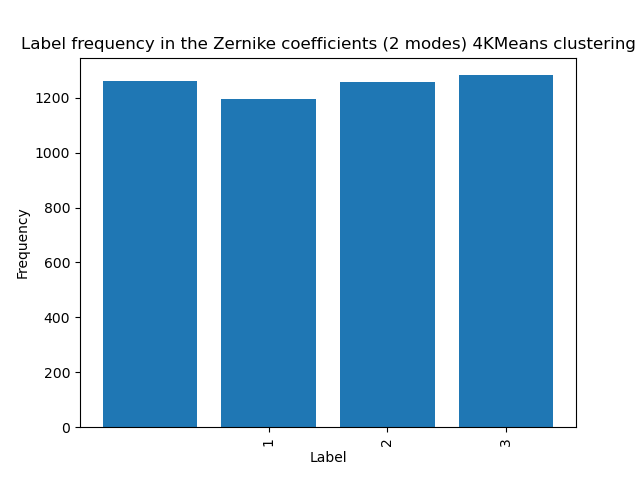
\includegraphics[width=0.2\textwidth]{nmia-zernikecoefficients(2modes)4KMeansdensity.png}}
			\hspace{\fill}
			\subfloat[4KMeans PSF Intensities UMAP]{%
				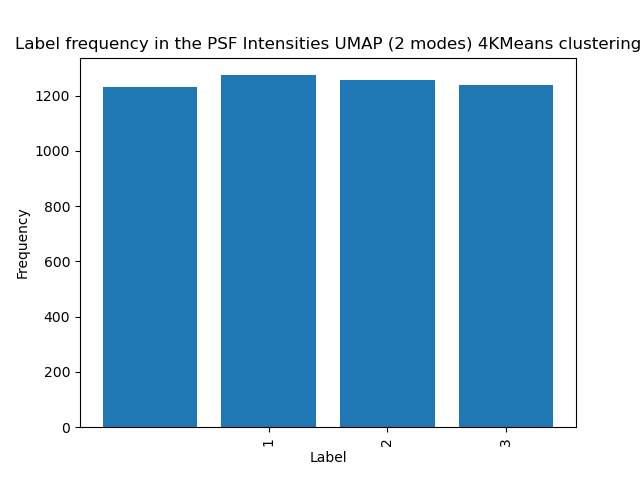
\includegraphics[width=0.2\textwidth]{nmia-psfintensitiesumap(2modes)4KMeansdensity.png}}
			\hspace{\fill}
			\subfloat[4KMeans LP coefficients]{%
				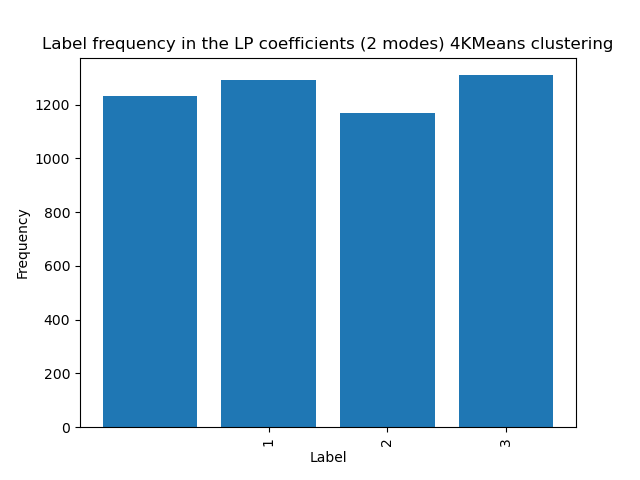
\includegraphics[width=0.2\textwidth]{nmia-lpcoefficients(2modes)4KMeansdensity.png}}
			\hspace{\fill}
			\subfloat[4KMeans Output Fluxes]{%
				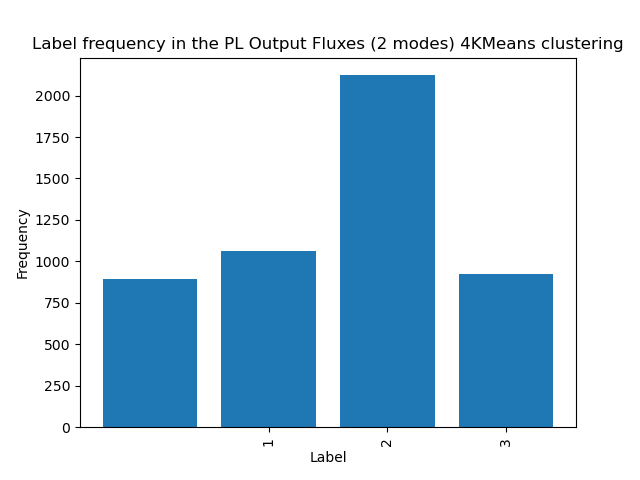
\includegraphics[width=0.2\textwidth]{nmia-ploutputfluxes(2modes)4KMeansdensity.png}}
		\end{figure*}
			
		\begin{figure*}[ht!]
			\centering	
			\subfloat[8KMeans for Zernike coefficients]{%
				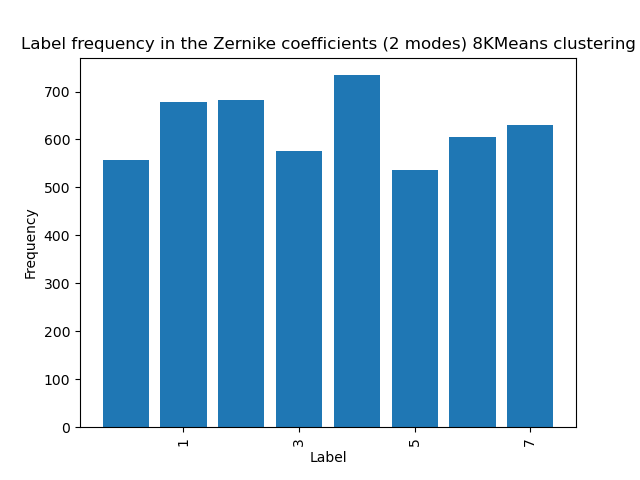
\includegraphics[width=0.2\textwidth]{nmia-zernikecoefficients(2modes)8KMeansdensity.png}}
			\hspace{\fill}
			\subfloat[8KMeans PSF Intensities UMAP]{%
				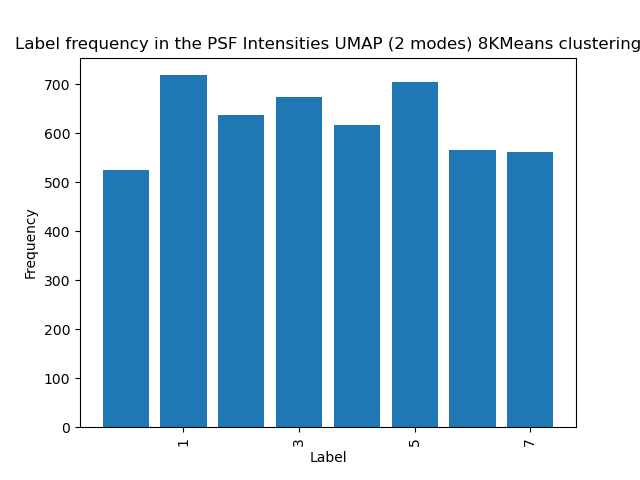
\includegraphics[width=0.2\textwidth]{nmia-psfintensitiesumap(2modes)8KMeansdensity.png}}
			\hspace{\fill}
			\subfloat[8KMeans LP coefficients]{%
				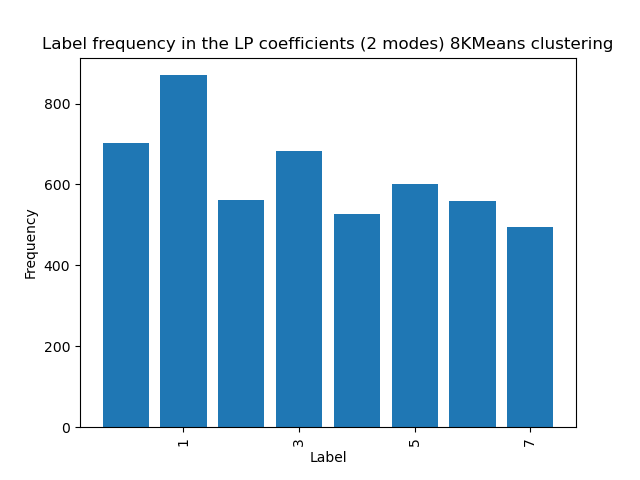
\includegraphics[width=0.2\textwidth]{nmia-lpcoefficients(2modes)8KMeansdensity.png}}
			\hspace{\fill}
			\subfloat[8KMeans Output Fluxes]{%
				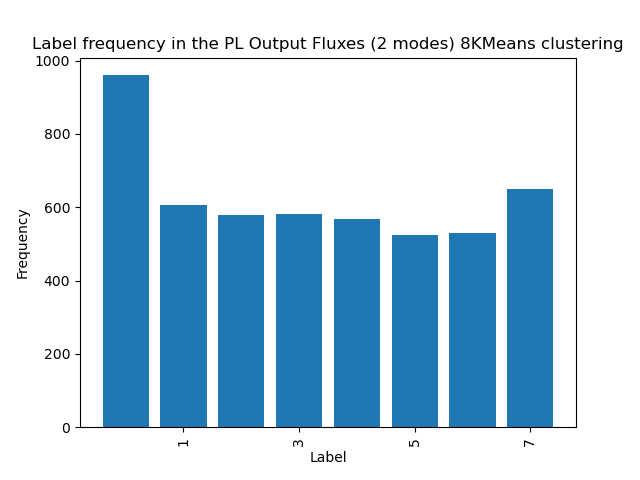
\includegraphics[width=0.2\textwidth]{nmia-ploutputfluxes(2modes)8KMeansdensity.png}}
		\end{figure*}
			
		\begin{figure*}[ht!]
			\centering	
			\subfloat[16KMeans for Zernike coefficients]{%
				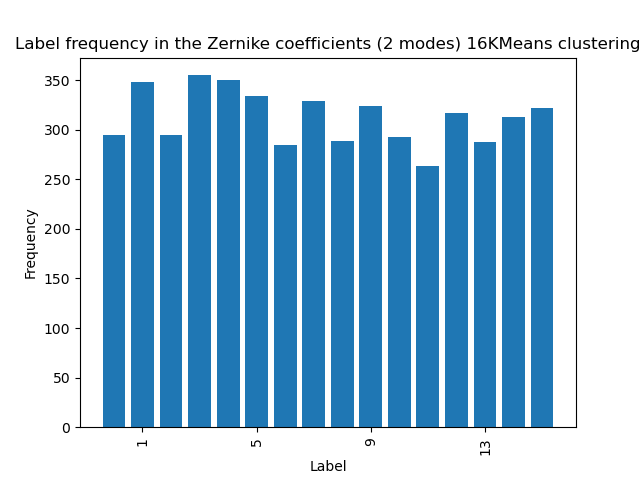
\includegraphics[width=0.2\textwidth]{nmia-zernikecoefficients(2modes)16KMeansdensity.png}}
			\hspace{\fill}
			\subfloat[16KMeans PSF Intensities UMAP]{%
				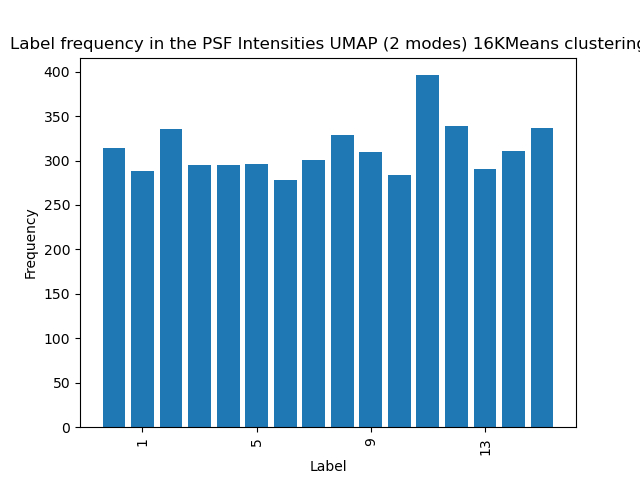
\includegraphics[width=0.2\textwidth]{nmia-psfintensitiesumap(2modes)16KMeansdensity.png}}
			\hspace{\fill}
			\subfloat[16KMeans LP coefficients]{%
				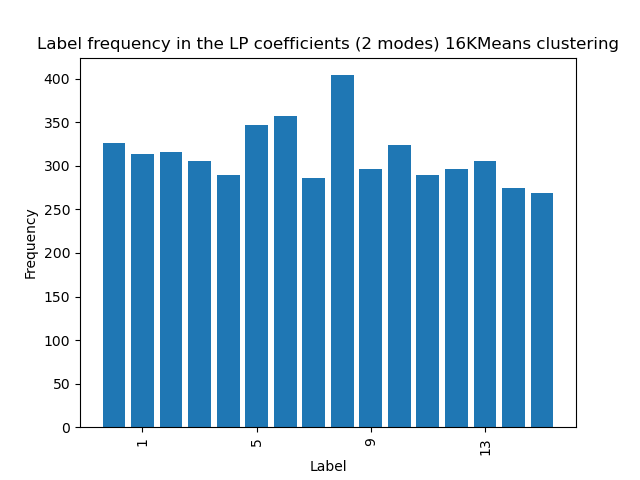
\includegraphics[width=0.2\textwidth]{nmia-lpcoefficients(2modes)16KMeansdensity.png}}
			\hspace{\fill}
			\subfloat[16KMeans Output Fluxes]{%
				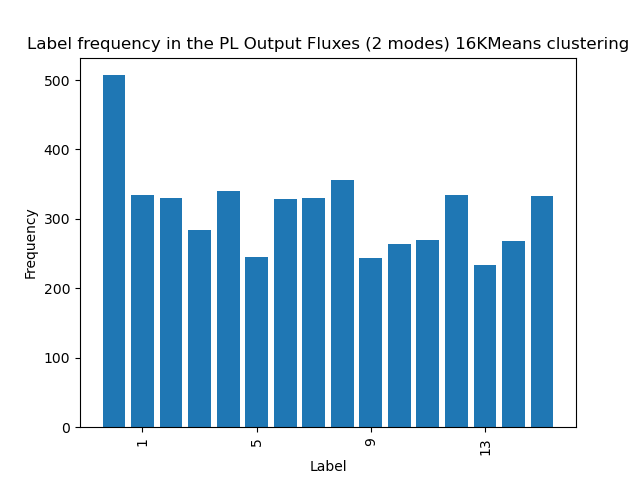
\includegraphics[width=0.2\textwidth]{nmia-ploutputfluxes(2modes)16KMeansdensity.png}}
		\end{figure*}
			
		\begin{figure*}[ht!]
			\centering
			\subfloat[32KMeans for Zernike coefficients]{%
				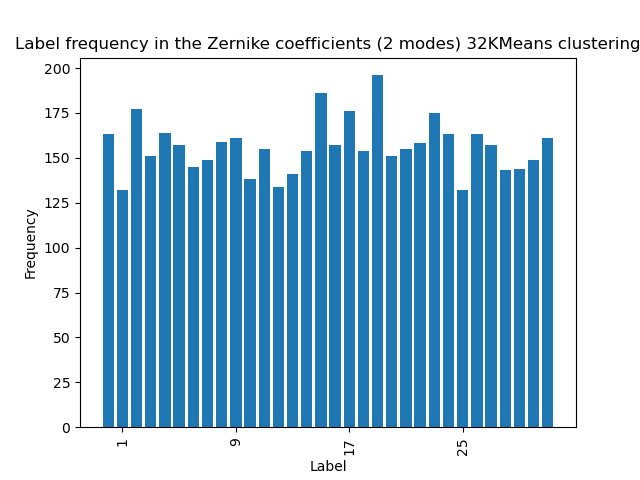
\includegraphics[width=0.2\textwidth]{nmia-zernikecoefficients(2modes)32KMeansdensity.png}}
			\hspace{\fill}
			\subfloat[32KMeans PSF Intensities UMAP]{%
				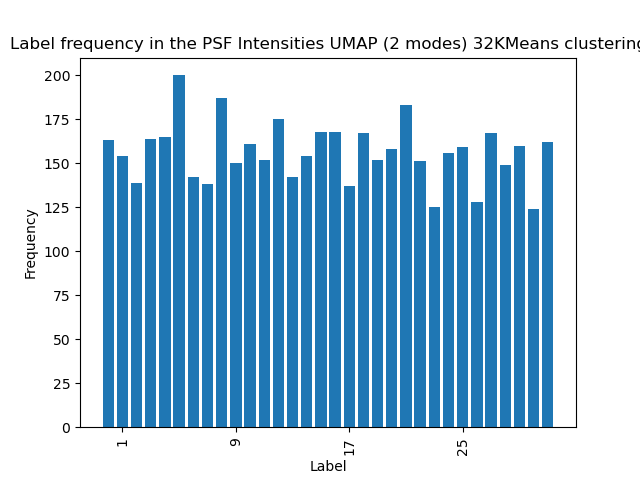
\includegraphics[width=0.2\textwidth]{nmia-psfintensitiesumap(2modes)32KMeansdensity.png}}
			\hspace{\fill}
			\subfloat[32KMeans LP coefficients]{%
				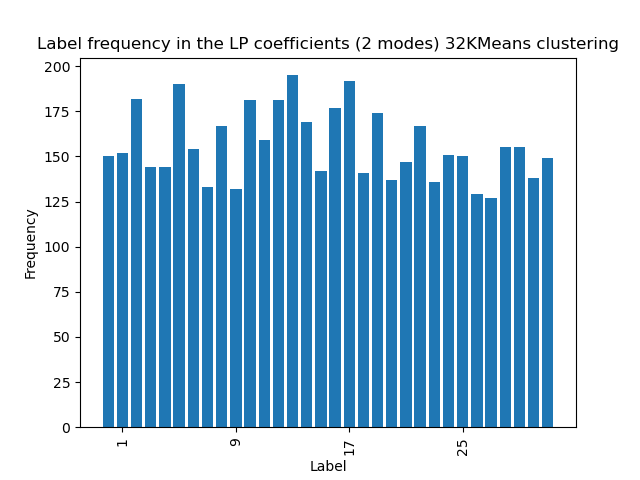
\includegraphics[width=0.2\textwidth]{nmia-lpcoefficients(2modes)32KMeansdensity.png}}
			\hspace{\fill}
			\subfloat[32KMeans Output Fluxes]{%
				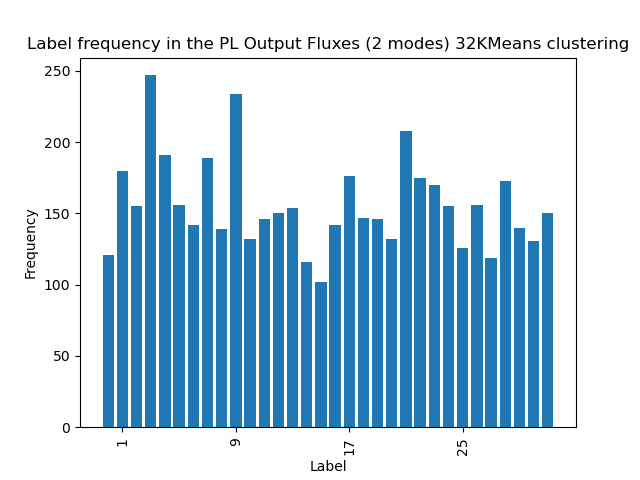
\includegraphics[width=0.2\textwidth]{nmia-ploutputfluxes(2modes)32KMeansdensity.png}}
		\end{figure*}
			
		\begin{figure*}[ht!]
			\centering	
			\subfloat[64KMeans for Zernike coefficients]{%
				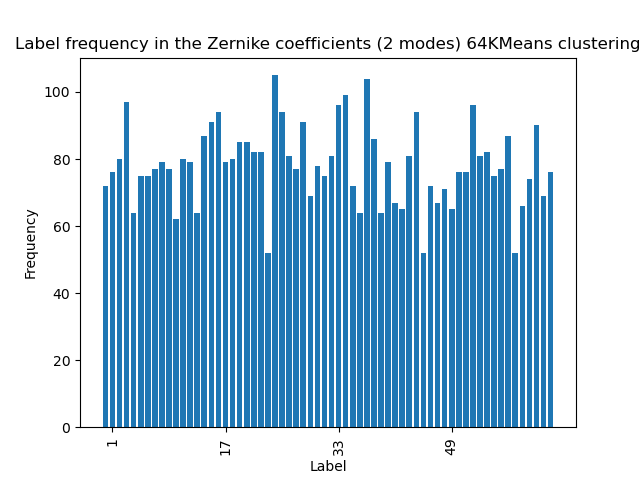
\includegraphics[width=0.2\textwidth]{nmia-zernikecoefficients(2modes)64KMeansdensity.png}}
			\hspace{\fill}
			\subfloat[64KMeans PSF Intensities UMAP]{%
				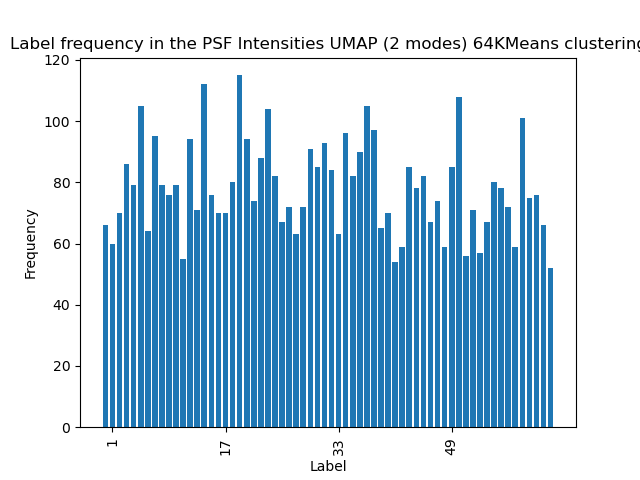
\includegraphics[width=0.2\textwidth]{nmia-psfintensitiesumap(2modes)64KMeansdensity.png}}
			\hspace{\fill}
			\subfloat[64KMeans LP coefficients]{%
				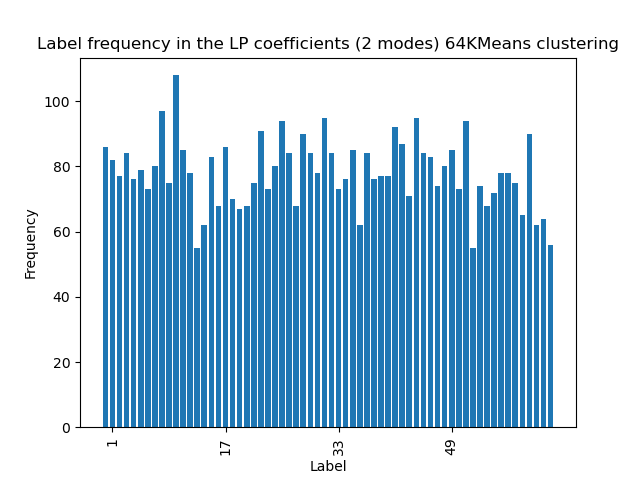
\includegraphics[width=0.2\textwidth]{nmia-lpcoefficients(2modes)64KMeansdensity.png}}
			\hspace{\fill}
			\subfloat[64KMeans Output Fluxes]{%
				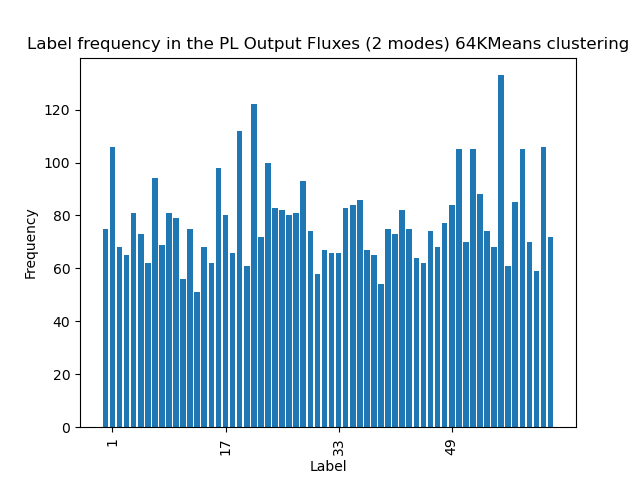
\includegraphics[width=0.2\textwidth]{nmia-ploutputfluxes(2modes)64KMeansdensity.png}}
		\end{figure*}
			
		\begin{figure*}[ht!]
			\centering	
			\subfloat[100KMeans for Zernike coefficients]{%
				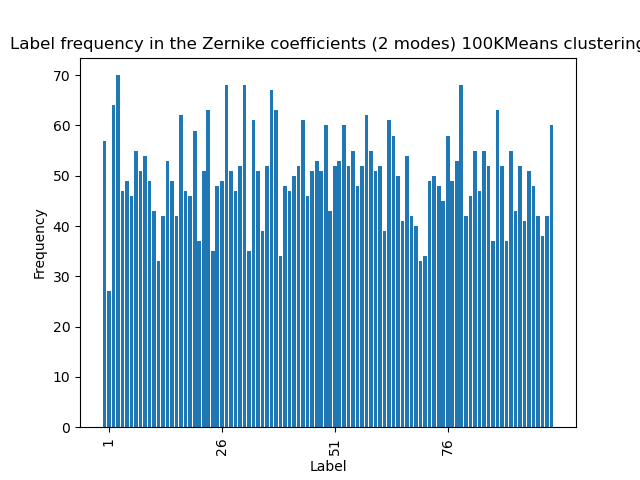
\includegraphics[width=0.2\textwidth]{nmia-zernikecoefficients(2modes)100KMeansdensity.png}}
			\hspace{\fill}
			\subfloat[100KMeans PSF Intensities UMAP]{%
				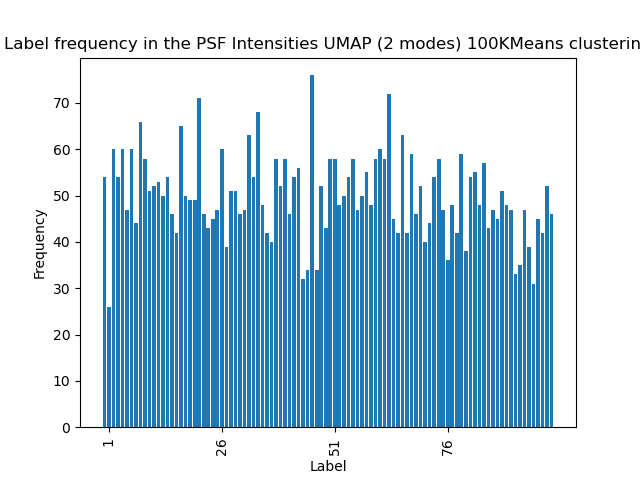
\includegraphics[width=0.2\textwidth]{nmia-psfintensitiesumap(2modes)100KMeansdensity.png}}
			\hspace{\fill}
			\subfloat[100KMeans LP coefficients]{%
				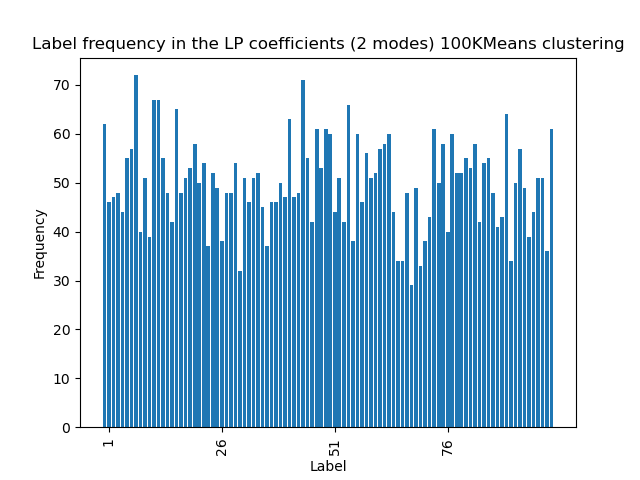
\includegraphics[width=0.2\textwidth]{nmia-lpcoefficients(2modes)100KMeansdensity.png}}
			\hspace{\fill}
			\subfloat[100KMeans Output Fluxes]{%
				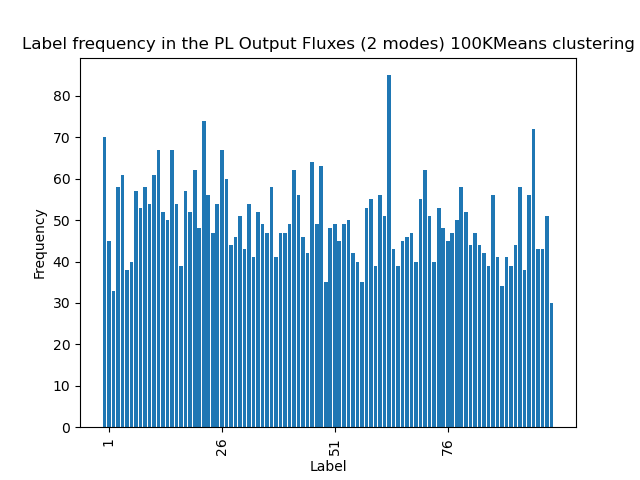
\includegraphics[width=0.2\textwidth]{nmia-ploutputfluxes(2modes)100KMeansdensity.png}}
		\end{figure*}
			
		\begin{figure*}[ht!]
			\centering	
			\subfloat[250KMeans for Zernike coefficients]{%
				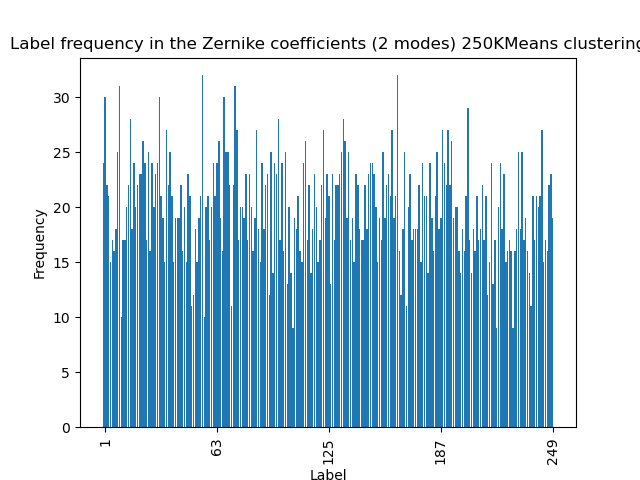
\includegraphics[width=0.2\textwidth]{nmia-zernikecoefficients(2modes)250KMeansdensity.png}}
			\hspace{\fill}
			\subfloat[250KMeans PSF Intensities UMAP]{%
				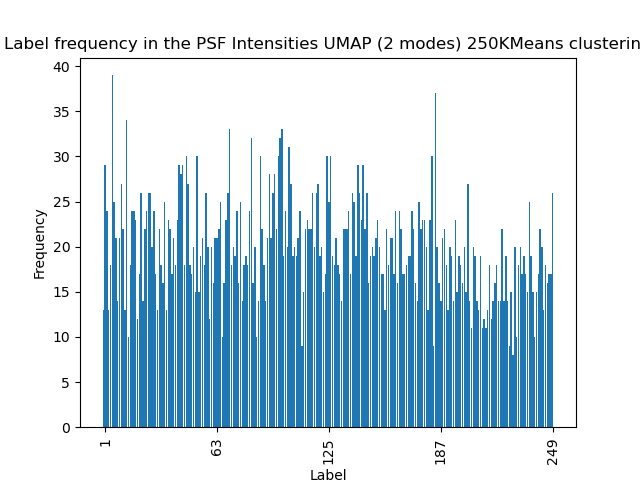
\includegraphics[width=0.2\textwidth]{nmia-psfintensitiesumap(2modes)250KMeansdensity.png}}
			\hspace{\fill}
			\subfloat[250KMeans LP coefficients]{%
				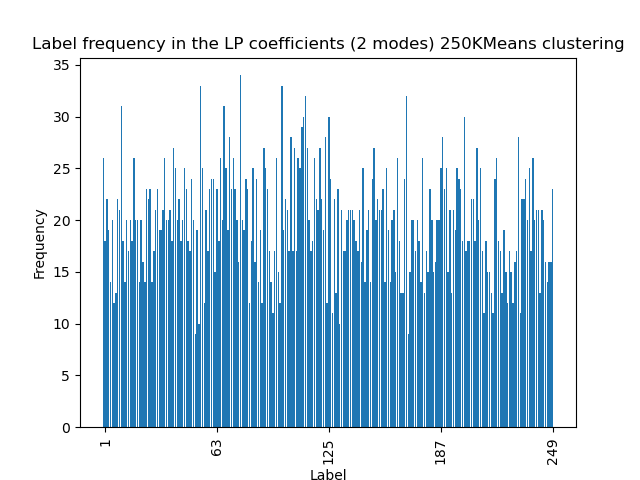
\includegraphics[width=0.2\textwidth]{nmia-lpcoefficients(2modes)250KMeansdensity.png}}
			\hspace{\fill}
			\subfloat[250KMeans Output Fluxes]{%
				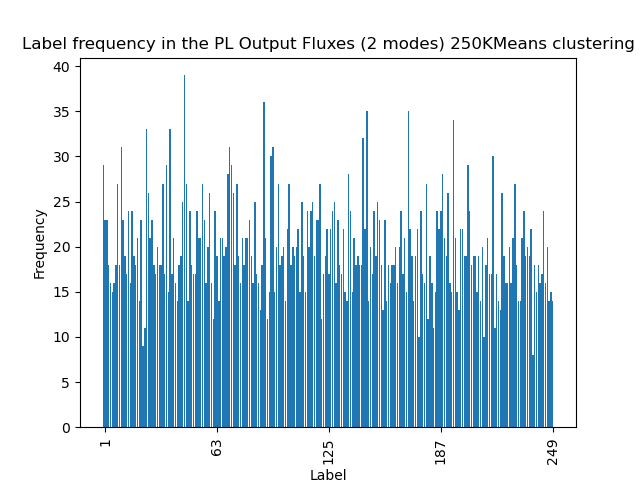
\includegraphics[width=0.2\textwidth]{nmia-ploutputfluxes(2modes)250KMeansdensity.png}}
		\end{figure*}
			
		\begin{figure*}[ht!]
			\centering	
			\subfloat[500KMeans for Zernike coefficients]{%
				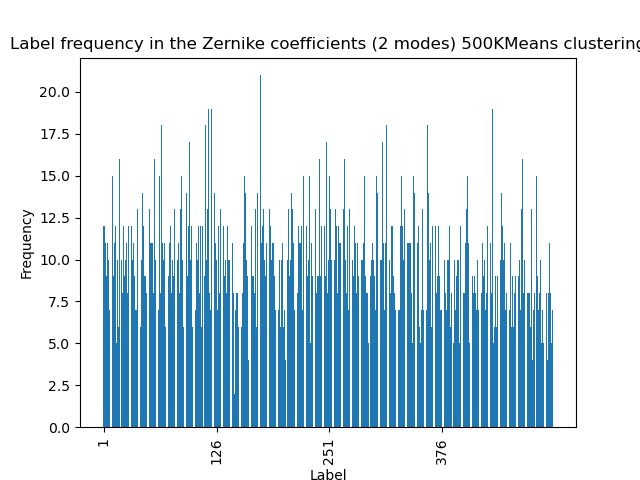
\includegraphics[width=0.2\textwidth]{nmia-zernikecoefficients(2modes)500KMeansdensity.png}}
			\hspace{\fill}
			\subfloat[500KMeans PSF Intensities UMAP]{%
				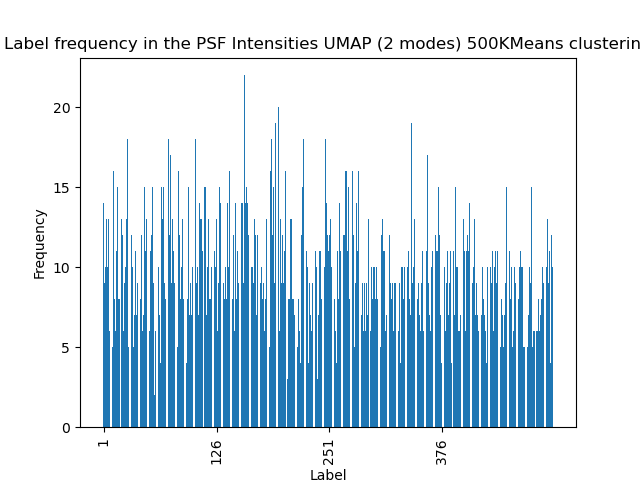
\includegraphics[width=0.2\textwidth]{nmia-psfintensitiesumap(2modes)500KMeansdensity.png}}
			\hspace{\fill}
			\subfloat[500KMeans LP coefficients]{%
				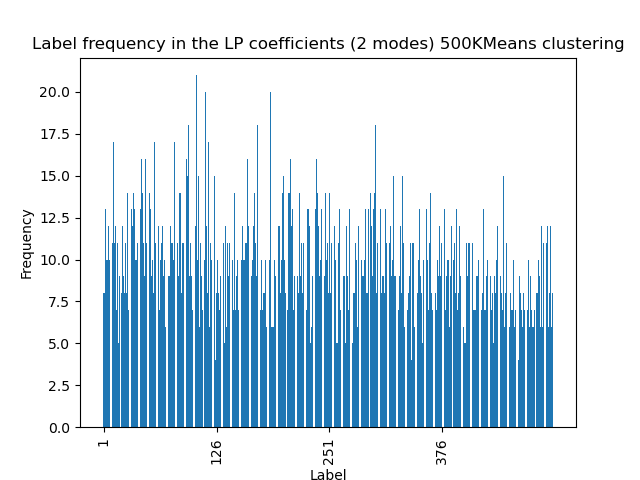
\includegraphics[width=0.2\textwidth]{nmia-lpcoefficients(2modes)500KMeansdensity.png}}
			\hspace{\fill}
			\subfloat[500KMeans Output Fluxes]{%
				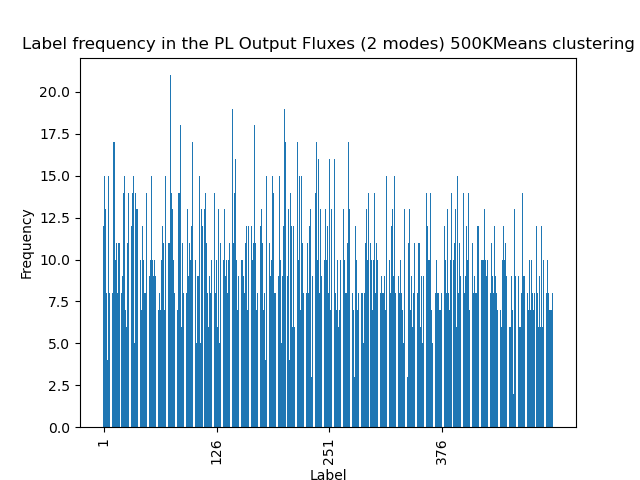
\includegraphics[width=0.2\textwidth]{nmia-ploutputfluxes(2modes)500KMeansdensity.png}}
		\end{figure*}
			
		\begin{figure*}[ht!]
			\centering	
			\subfloat[1000KMeans for Zernike coefficients]{%
				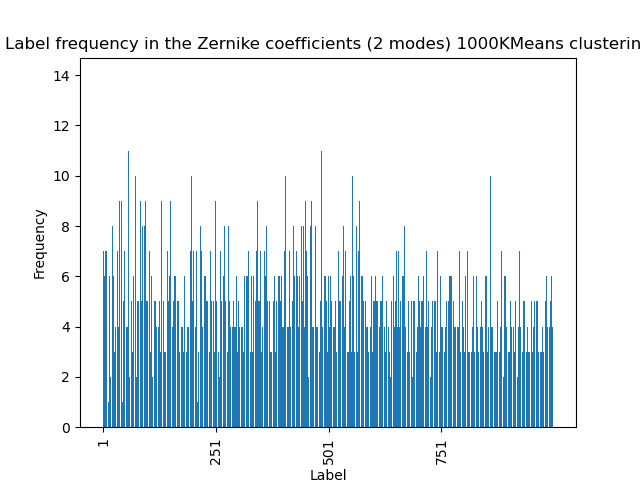
\includegraphics[width=0.2\textwidth]{nmia-zernikecoefficients(2modes)1000KMeansdensity.png}}
			\hspace{\fill}
			\subfloat[1000KMeans PSF Intensities UMAP]{%
				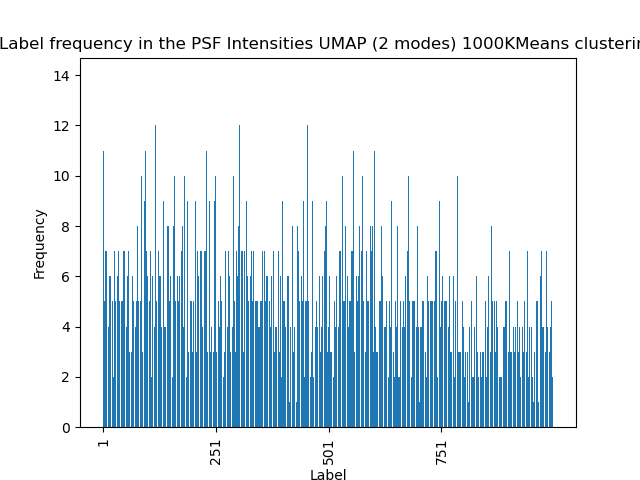
\includegraphics[width=0.2\textwidth]{nmia-psfintensitiesumap(2modes)1000KMeansdensity.png}}
			\hspace{\fill}
			\subfloat[1000KMeans LP coefficients]{%
				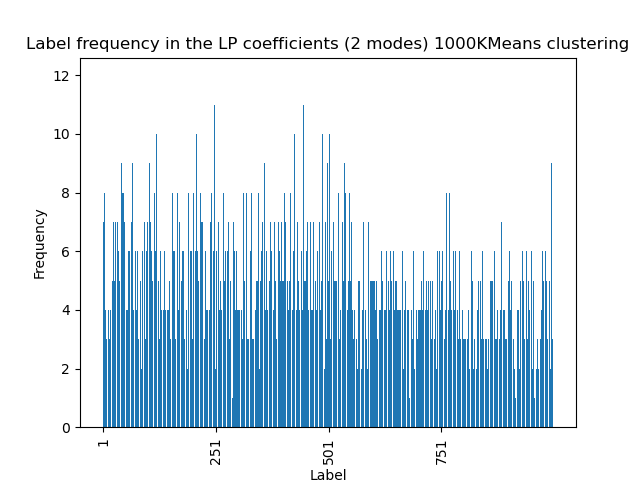
\includegraphics[width=0.2\textwidth]{nmia-lpcoefficients(2modes)1000KMeansdensity.png}}
			\hspace{\fill}
			\subfloat[1000KMeans Output Fluxes]{%
				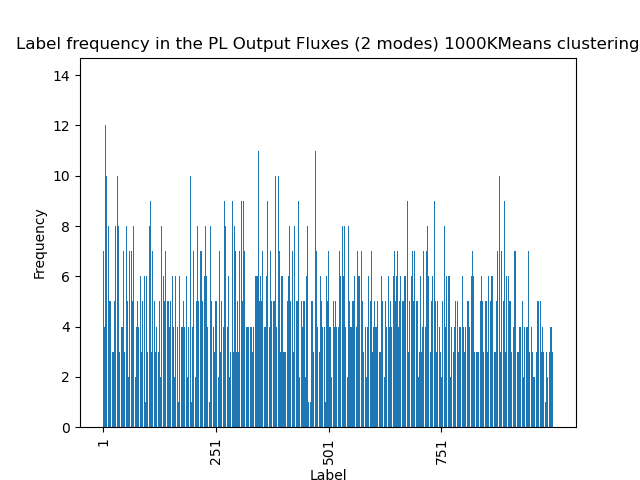
\includegraphics[width=0.2\textwidth]{nmia-ploutputfluxes(2modes)1000KMeansdensity.png}}
		\end{figure*}
		\FloatBarrier
		
		\subsubsection{5 Zernike modes datasets clusters densities}
		
		\begin{figure*}[ht!]
			\centering
			\subfloat[4KMeans for Zernike coefficients]{%
				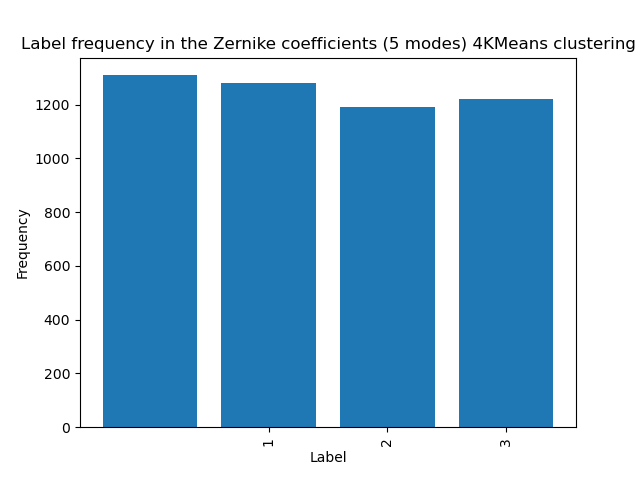
\includegraphics[width=0.2\textwidth]{nmia-zernikecoefficients(5modes)4KMeansdensity.png}}
			\hspace{\fill}
			\subfloat[4KMeans PSF Intensities UMAP]{%
				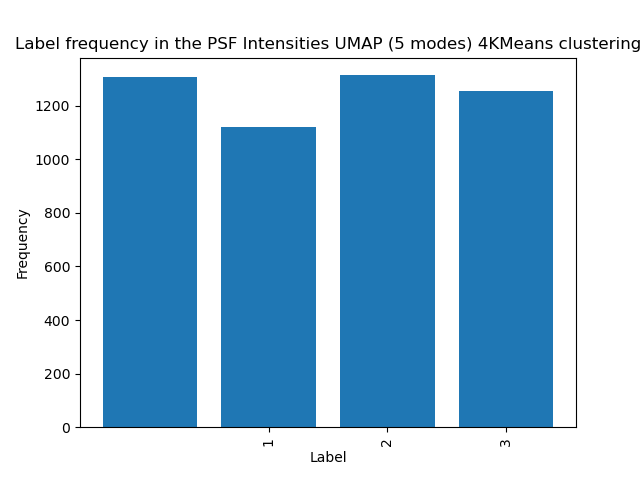
\includegraphics[width=0.2\textwidth]{nmia-psfintensitiesumap(5modes)4KMeansdensity.png}}
			\hspace{\fill}
			\subfloat[4KMeans LP coefficients]{%
				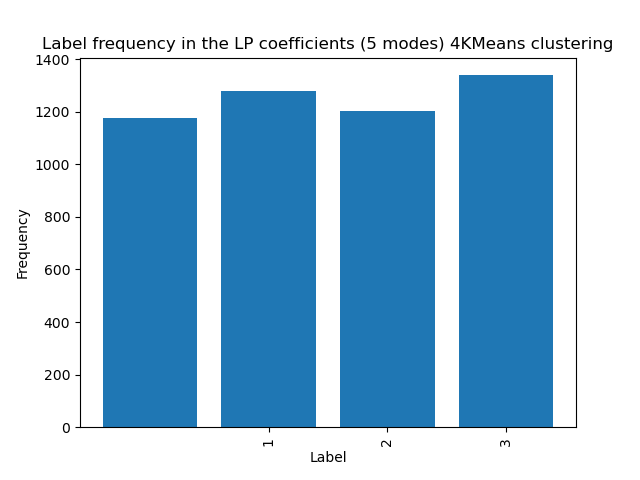
\includegraphics[width=0.2\textwidth]{nmia-lpcoefficients(5modes)4KMeansdensity.png}}
			\hspace{\fill}
			\subfloat[4KMeans Output Fluxes]{%
				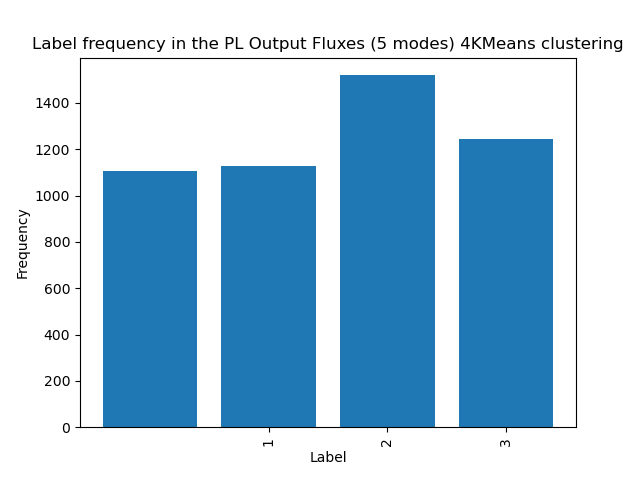
\includegraphics[width=0.2\textwidth]{nmia-ploutputfluxes(5modes)4KMeansdensity.png}}
		\end{figure*}
			
		\begin{figure*}[ht!]
			\centering	
			\subfloat[8KMeans for Zernike coefficients]{%
				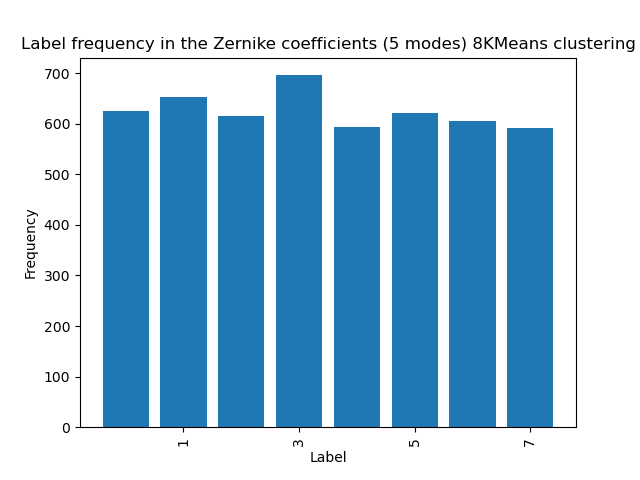
\includegraphics[width=0.2\textwidth]{nmia-zernikecoefficients(5modes)8KMeansdensity.png}}
			\hspace{\fill}
			\subfloat[8KMeans PSF Intensities UMAP]{%
				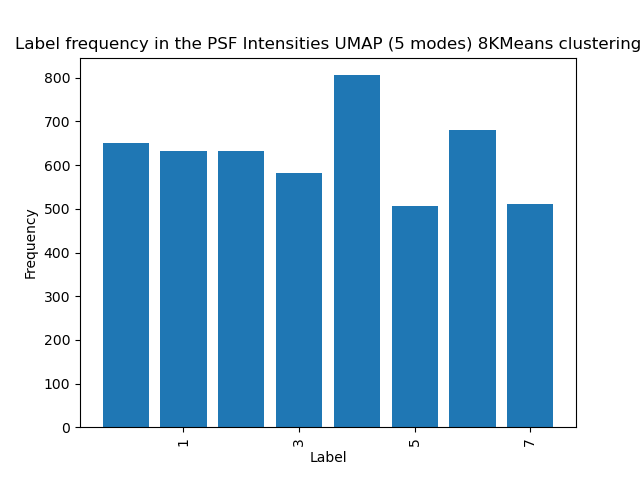
\includegraphics[width=0.2\textwidth]{nmia-psfintensitiesumap(5modes)8KMeansdensity.png}}
			\hspace{\fill}
			\subfloat[8KMeans LP coefficients]{%
				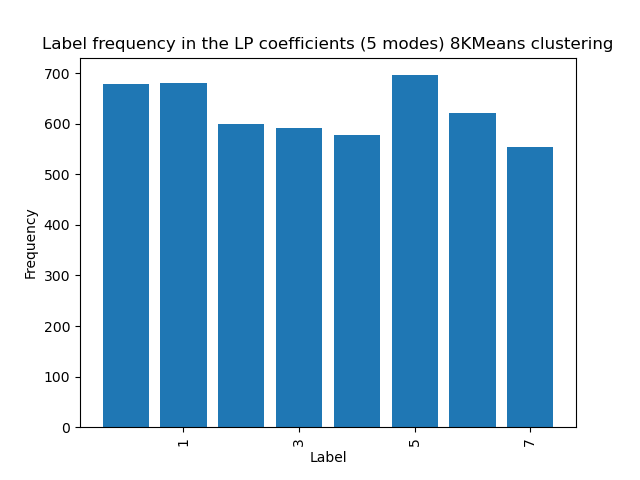
\includegraphics[width=0.2\textwidth]{nmia-lpcoefficients(5modes)8KMeansdensity.png}}
			\hspace{\fill}
			\subfloat[8KMeans Output Fluxes]{%
				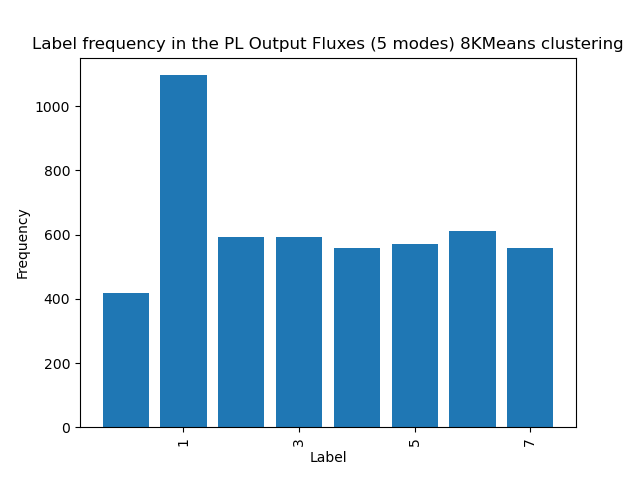
\includegraphics[width=0.2\textwidth]{nmia-ploutputfluxes(5modes)8KMeansdensity.png}}
		\end{figure*}
			
		\begin{figure*}[ht!]
			\centering	
			\subfloat[16KMeans for Zernike coefficients]{%
				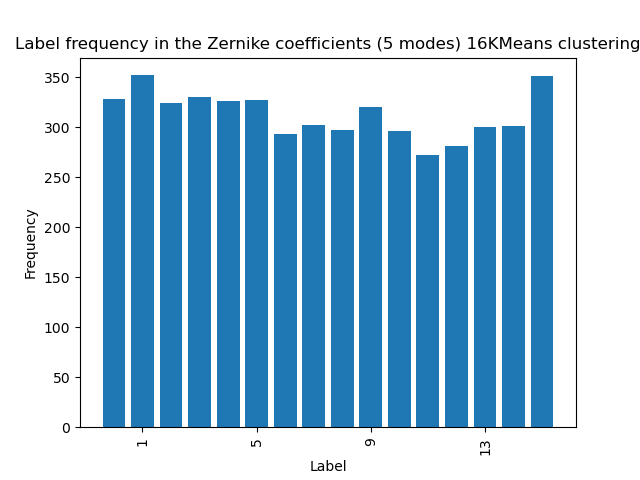
\includegraphics[width=0.2\textwidth]{nmia-zernikecoefficients(5modes)16KMeansdensity.png}}
			\hspace{\fill}
			\subfloat[16KMeans PSF Intensities UMAP]{%
				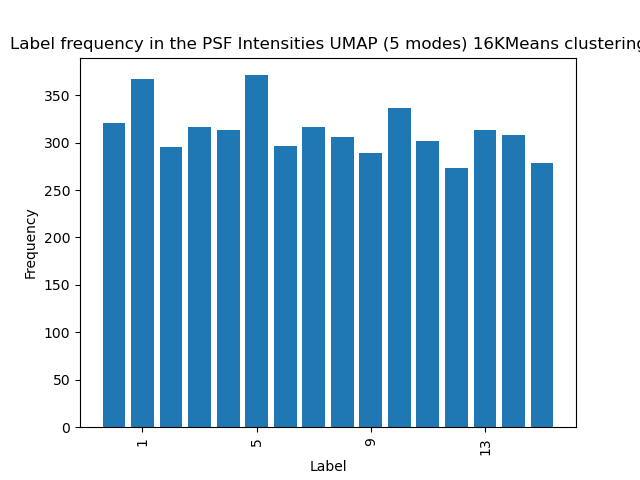
\includegraphics[width=0.2\textwidth]{nmia-psfintensitiesumap(5modes)16KMeansdensity.png}}
			\hspace{\fill}
			\subfloat[16KMeans LP coefficients]{%
				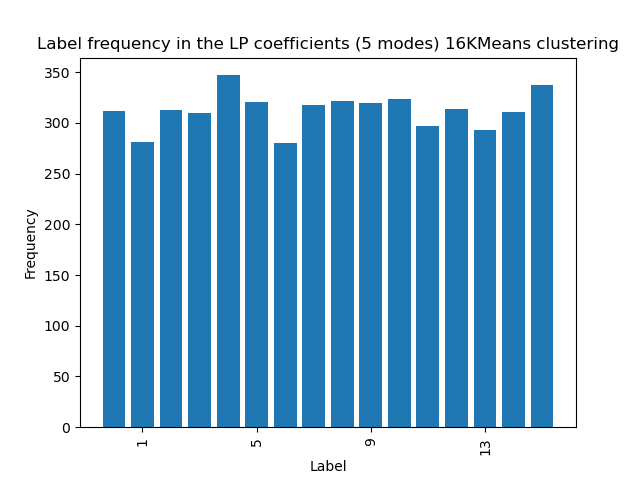
\includegraphics[width=0.2\textwidth]{nmia-lpcoefficients(5modes)16KMeansdensity.png}}
			\hspace{\fill}
			\subfloat[16KMeans Output Fluxes]{%
				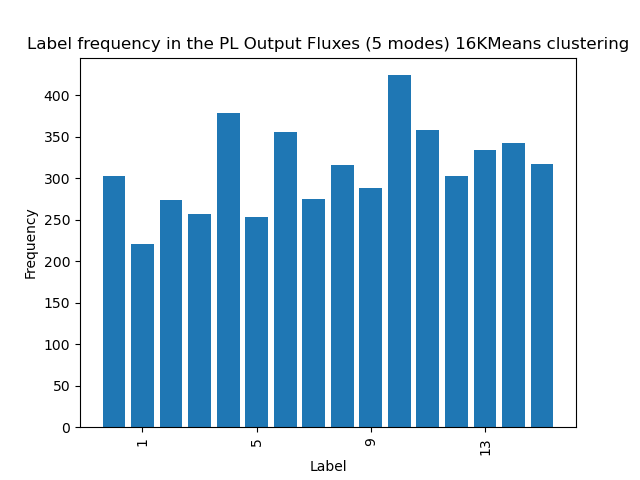
\includegraphics[width=0.2\textwidth]{nmia-ploutputfluxes(5modes)16KMeansdensity.png}}
		\end{figure*}
			
		\begin{figure*}[ht!]
			\centering
			\subfloat[32KMeans for Zernike coefficients]{%
				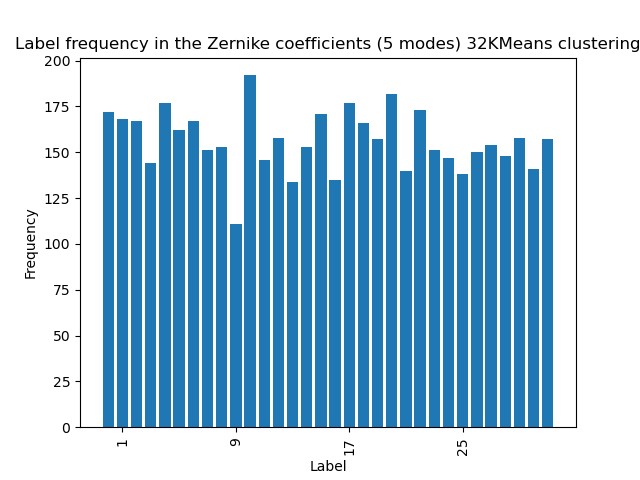
\includegraphics[width=0.2\textwidth]{nmia-zernikecoefficients(5modes)32KMeansdensity.png}}
			\hspace{\fill}
			\subfloat[32KMeans PSF Intensities UMAP]{%
				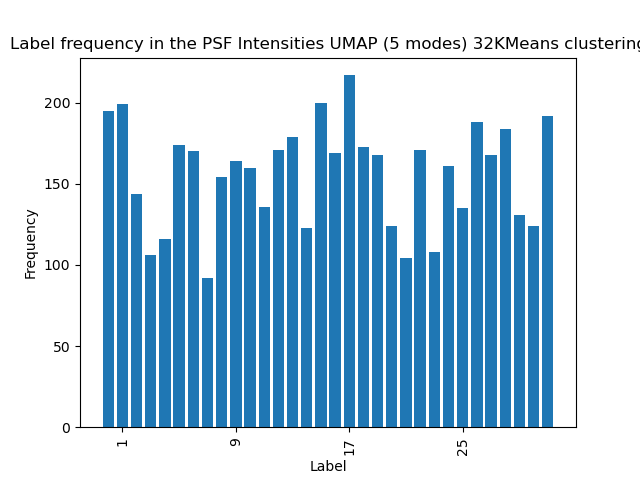
\includegraphics[width=0.2\textwidth]{nmia-psfintensitiesumap(5modes)32KMeansdensity.png}}
			\hspace{\fill}
			\subfloat[32KMeans LP coefficients]{%
				\includegraphics[width=0.2\textwidth]{nmia-lpcoefficients(5modes)32KMeansdensity.png}}
			\hspace{\fill}
			\subfloat[32KMeans Output Fluxes]{%
				\includegraphics[width=0.2\textwidth]{nmia-ploutputfluxes(5modes)32KMeansdensity.png}}
		\end{figure*}
			
		\begin{figure*}[ht!]
			\centering	
			\subfloat[64KMeans for Zernike coefficients]{%
				\includegraphics[width=0.2\textwidth]{nmia-zernikecoefficients(5modes)64KMeansdensity.png}}
			\hspace{\fill}
			\subfloat[64KMeans PSF Intensities UMAP]{%
				\includegraphics[width=0.2\textwidth]{nmia-psfintensitiesumap(5modes)64KMeansdensity.png}}
			\hspace{\fill}
			\subfloat[64KMeans LP coefficients]{%
				\includegraphics[width=0.2\textwidth]{nmia-lpcoefficients(5modes)64KMeansdensity.png}}
			\hspace{\fill}
			\subfloat[64KMeans Output Fluxes]{%
				\includegraphics[width=0.2\textwidth]{nmia-ploutputfluxes(5modes)64KMeansdensity.png}}
		\end{figure*}
			
		\begin{figure*}[ht!]
			\centering	
			\subfloat[100KMeans for Zernike coefficients]{%
				\includegraphics[width=0.2\textwidth]{nmia-zernikecoefficients(5modes)100KMeansdensity.png}}
			\hspace{\fill}
			\subfloat[100KMeans PSF Intensities UMAP]{%
				\includegraphics[width=0.2\textwidth]{nmia-psfintensitiesumap(5modes)100KMeansdensity.png}}
			\hspace{\fill}
			\subfloat[100KMeans LP coefficients]{%
				\includegraphics[width=0.2\textwidth]{nmia-lpcoefficients(5modes)100KMeansdensity.png}}
			\hspace{\fill}
			\subfloat[100KMeans Output Fluxes]{%
				\includegraphics[width=0.2\textwidth]{nmia-ploutputfluxes(5modes)100KMeansdensity.png}}
		\end{figure*}
			
		\begin{figure*}[ht!]
			\centering	
			\subfloat[250KMeans for Zernike coefficients]{%
				\includegraphics[width=0.2\textwidth]{nmia-zernikecoefficients(5modes)250KMeansdensity.png}}
			\hspace{\fill}
			\subfloat[250KMeans PSF Intensities UMAP]{%
				\includegraphics[width=0.2\textwidth]{nmia-psfintensitiesumap(5modes)250KMeansdensity.png}}
			\hspace{\fill}
			\subfloat[250KMeans LP coefficients]{%
				\includegraphics[width=0.2\textwidth]{nmia-lpcoefficients(5modes)250KMeansdensity.png}}
			\hspace{\fill}
			\subfloat[250KMeans Output Fluxes]{%
				\includegraphics[width=0.2\textwidth]{nmia-ploutputfluxes(5modes)250KMeansdensity.png}}
		\end{figure*}
			
		\begin{figure*}[ht!]
			\centering	
			\subfloat[500KMeans for Zernike coefficients]{%
				\includegraphics[width=0.2\textwidth]{nmia-zernikecoefficients(5modes)500KMeansdensity.png}}
			\hspace{\fill}
			\subfloat[500KMeans PSF Intensities UMAP]{%
				\includegraphics[width=0.2\textwidth]{nmia-psfintensitiesumap(5modes)500KMeansdensity.png}}
			\hspace{\fill}
			\subfloat[500KMeans LP coefficients]{%
				\includegraphics[width=0.2\textwidth]{nmia-lpcoefficients(5modes)500KMeansdensity.png}}
			\hspace{\fill}
			\subfloat[500KMeans Output Fluxes]{%
				\includegraphics[width=0.2\textwidth]{nmia-ploutputfluxes(5modes)500KMeansdensity.png}}
		\end{figure*}
			
		\begin{figure*}[ht!]
			\centering	
			\subfloat[1000KMeans for Zernike coefficients]{%
				\includegraphics[width=0.2\textwidth]{nmia-zernikecoefficients(5modes)1000KMeansdensity.png}}
			\hspace{\fill}
			\subfloat[250KMeans PSF Intensities UMAP]{%
				\includegraphics[width=0.2\textwidth]{nmia-psfintensitiesumap(5modes)1000KMeansdensity.png}}
			\hspace{\fill}
			\subfloat[250KMeans LP coefficients]{%
				\includegraphics[width=0.2\textwidth]{nmia-lpcoefficients(5modes)1000KMeansdensity.png}}
			\hspace{\fill}
			\subfloat[250KMeans Output Fluxes]{%
				\includegraphics[width=0.2\textwidth]{nmia-ploutputfluxes(5modes)1000KMeansdensity.png}}
		\end{figure*}
		\FloatBarrier
		
		
		\subsubsection{9 Zernike modes datasets clusters densities}
		
		\begin{figure*}[ht!]
			\centering
			\subfloat[4KMeans for Zernike coefficients]{%
				\includegraphics[width=0.2\textwidth]{nmia-zernikecoefficients(9modes)4KMeansdensity.png}}
			\hspace{\fill}
			\subfloat[4KMeans PSF Intensities UMAP]{%
				\includegraphics[width=0.2\textwidth]{nmia-psfintensitiesumap(9modes)4KMeansdensity.png}}
			\hspace{\fill}
			\subfloat[4KMeans LP coefficients]{%
				\includegraphics[width=0.2\textwidth]{nmia-lpcoefficients(9modes)4KMeansdensity.png}}
			\hspace{\fill}
			\subfloat[4KMeans Output Fluxes]{%
				\includegraphics[width=0.2\textwidth]{nmia-ploutputfluxes(9modes)4KMeansdensity.png}}
		\end{figure*}
			
		\begin{figure*}[ht!]
			\centering	
			\subfloat[8KMeans for Zernike coefficients]{%
				\includegraphics[width=0.2\textwidth]{nmia-zernikecoefficients(9modes)8KMeansdensity.png}}
			\hspace{\fill}
			\subfloat[8KMeans PSF Intensities UMAP]{%
				\includegraphics[width=0.2\textwidth]{nmia-psfintensitiesumap(9modes)8KMeansdensity.png}}
			\hspace{\fill}
			\subfloat[8KMeans LP coefficients]{%
				\includegraphics[width=0.2\textwidth]{nmia-lpcoefficients(9modes)8KMeansdensity.png}}
			\hspace{\fill}
			\subfloat[8KMeans Output Fluxes]{%
				\includegraphics[width=0.2\textwidth]{nmia-ploutputfluxes(9modes)8KMeansdensity.png}}
		\end{figure*}
			
		\begin{figure*}[ht!]
			\centering	
			\subfloat[16KMeans for Zernike coefficients]{%
				\includegraphics[width=0.2\textwidth]{nmia-zernikecoefficients(9modes)16KMeansdensity.png}}
			\hspace{\fill}
			\subfloat[16KMeans PSF Intensities UMAP]{%
				\includegraphics[width=0.2\textwidth]{nmia-psfintensitiesumap(9modes)16KMeansdensity.png}}
			\hspace{\fill}
			\subfloat[16KMeans LP coefficients]{%
				\includegraphics[width=0.2\textwidth]{nmia-lpcoefficients(9modes)16KMeansdensity.png}}
			\hspace{\fill}
			\subfloat[16KMeans Output Fluxes]{%
				\includegraphics[width=0.2\textwidth]{nmia-ploutputfluxes(9modes)16KMeansdensity.png}}
		\end{figure*}
			
		\begin{figure*}[ht!]
			\centering
			\subfloat[32KMeans for Zernike coefficients]{%
				\includegraphics[width=0.2\textwidth]{nmia-zernikecoefficients(9modes)32KMeansdensity.png}}
			\hspace{\fill}
			\subfloat[32KMeans PSF Intensities UMAP]{%
				\includegraphics[width=0.2\textwidth]{nmia-psfintensitiesumap(9modes)32KMeansdensity.png}}
			\hspace{\fill}
			\subfloat[32KMeans LP coefficients]{%
				\includegraphics[width=0.2\textwidth]{nmia-lpcoefficients(9modes)32KMeansdensity.png}}
			\hspace{\fill}
			\subfloat[32KMeans Output Fluxes]{%
				\includegraphics[width=0.2\textwidth]{nmia-ploutputfluxes(9modes)32KMeansdensity.png}}
		\end{figure*}
			
		\begin{figure*}[ht!]
			\centering	
			\subfloat[64KMeans for Zernike coefficients]{%
				\includegraphics[width=0.2\textwidth]{nmia-zernikecoefficients(9modes)64KMeansdensity.png}}
			\hspace{\fill}
			\subfloat[64KMeans PSF Intensities UMAP]{%
				\includegraphics[width=0.2\textwidth]{nmia-psfintensitiesumap(9modes)64KMeansdensity.png}}
			\hspace{\fill}
			\subfloat[64KMeans LP coefficients]{%
				\includegraphics[width=0.2\textwidth]{nmia-lpcoefficients(9modes)64KMeansdensity.png}}
			\hspace{\fill}
			\subfloat[64KMeans Output Fluxes]{%
				\includegraphics[width=0.2\textwidth]{nmia-ploutputfluxes(9modes)64KMeansdensity.png}}
		\end{figure*}
			
		\begin{figure*}[ht!]
			\centering	
			\subfloat[100KMeans for Zernike coefficients]{%
				\includegraphics[width=0.2\textwidth]{nmia-zernikecoefficients(9modes)100KMeansdensity.png}}
			\hspace{\fill}
			\subfloat[100KMeans PSF Intensities UMAP]{%
				\includegraphics[width=0.2\textwidth]{nmia-psfintensitiesumap(9modes)100KMeansdensity.png}}
			\hspace{\fill}
			\subfloat[100KMeans LP coefficients]{%
				\includegraphics[width=0.2\textwidth]{nmia-lpcoefficients(9modes)100KMeansdensity.png}}
			\hspace{\fill}
			\subfloat[100KMeans Output Fluxes]{%
				\includegraphics[width=0.2\textwidth]{nmia-ploutputfluxes(9modes)100KMeansdensity.png}}
		\end{figure*}
			
		\begin{figure*}[ht!]
			\centering	
			\subfloat[250KMeans for Zernike coefficients]{%
				\includegraphics[width=0.2\textwidth]{nmia-zernikecoefficients(9modes)250KMeansdensity.png}}
			\hspace{\fill}
			\subfloat[250KMeans PSF Intensities UMAP]{%
				\includegraphics[width=0.2\textwidth]{nmia-psfintensitiesumap(9modes)250KMeansdensity.png}}
			\hspace{\fill}
			\subfloat[250KMeans LP coefficients]{%
				\includegraphics[width=0.2\textwidth]{nmia-lpcoefficients(9modes)250KMeansdensity.png}}
			\hspace{\fill}
			\subfloat[250KMeans Output Fluxes]{%
				\includegraphics[width=0.2\textwidth]{nmia-ploutputfluxes(9modes)250KMeansdensity.png}}
		\end{figure*}
			
		\begin{figure*}[ht!]
			\centering	
			\subfloat[500KMeans for Zernike coefficients]{%
				\includegraphics[width=0.2\textwidth]{nmia-zernikecoefficients(9modes)500KMeansdensity.png}}
			\hspace{\fill}
			\subfloat[500KMeans PSF Intensities UMAP]{%
				\includegraphics[width=0.2\textwidth]{nmia-psfintensitiesumap(9modes)500KMeansdensity.png}}
			\hspace{\fill}
			\subfloat[500KMeans LP coefficients]{%
				\includegraphics[width=0.2\textwidth]{nmia-lpcoefficients(9modes)500KMeansdensity.png}}
			\hspace{\fill}
			\subfloat[500KMeans Output Fluxes]{%
				\includegraphics[width=0.2\textwidth]{nmia-ploutputfluxes(9modes)500KMeansdensity.png}}
		\end{figure*}
			
		\begin{figure*}[ht!]
			\centering	
			\subfloat[1000KMeans for Zernike coefficients]{%
				\includegraphics[width=0.2\textwidth]{nmia-zernikecoefficients(9modes)1000KMeansdensity.png}}
			\hspace{\fill}
			\subfloat[1000KMeans PSF Intensities UMAP]{%
				\includegraphics[width=0.2\textwidth]{nmia-psfintensitiesumap(9modes)1000KMeansdensity.png}}
			\hspace{\fill}
			\subfloat[1000KMeans LP coefficients]{%
				\includegraphics[width=0.2\textwidth]{nmia-lpcoefficients(9modes)1000KMeansdensity.png}}
			\hspace{\fill}
			\subfloat[1000KMeans Output Fluxes]{%
				\includegraphics[width=0.2\textwidth]{nmia-ploutputfluxes(9modes)1000KMeansdensity.png}}
		\end{figure*}
		\FloatBarrier
		
		
		\subsubsection{14 Zernike modes datasets clusters densities}
		
		\begin{figure*}[ht!]
			\centering
			\subfloat[4KMeans for Zernike coefficients]{%
				\includegraphics[width=0.2\textwidth]{nmia-zernikecoefficients(14modes)4KMeansdensity.png}}
			\hspace{\fill}
			\subfloat[4KMeans PSF Intensities UMAP]{%
				\includegraphics[width=0.2\textwidth]{nmia-psfintensitiesumap(14modes)4KMeansdensity.png}}
			\hspace{\fill}
			\subfloat[4KMeans LP coefficients]{%
				\includegraphics[width=0.2\textwidth]{nmia-lpcoefficients(14modes)4KMeansdensity.png}}
			\hspace{\fill}
			\subfloat[4KMeans Output Fluxes]{%
				\includegraphics[width=0.2\textwidth]{nmia-ploutputfluxes(14modes)4KMeansdensity.png}}
		\end{figure*}
			
		\begin{figure*}[ht!]
			\centering	
			\subfloat[8KMeans for Zernike coefficients]{%
				\includegraphics[width=0.2\textwidth]{nmia-zernikecoefficients(14modes)8KMeansdensity.png}}
			\hspace{\fill}
			\subfloat[8KMeans PSF Intensities UMAP]{%
				\includegraphics[width=0.2\textwidth]{nmia-psfintensitiesumap(14modes)8KMeansdensity.png}}
			\hspace{\fill}
			\subfloat[8KMeans LP coefficients]{%
				\includegraphics[width=0.2\textwidth]{nmia-lpcoefficients(14modes)8KMeansdensity.png}}
			\hspace{\fill}
			\subfloat[8KMeans Output Fluxes]{%
				\includegraphics[width=0.2\textwidth]{nmia-ploutputfluxes(14modes)8KMeansdensity.png}}
		\end{figure*}
			
		\begin{figure*}[ht!]
			\centering	
			\subfloat[16KMeans for Zernike coefficients]{%
				\includegraphics[width=0.2\textwidth]{nmia-zernikecoefficients(14modes)16KMeansdensity.png}}
			\hspace{\fill}
			\subfloat[16KMeans PSF Intensities UMAP]{%
				\includegraphics[width=0.2\textwidth]{nmia-psfintensitiesumap(14modes)16KMeansdensity.png}}
			\hspace{\fill}
			\subfloat[16KMeans LP coefficients]{%
				\includegraphics[width=0.2\textwidth]{nmia-lpcoefficients(14modes)16KMeansdensity.png}}
			\hspace{\fill}
			\subfloat[16KMeans Output Fluxes]{%
				\includegraphics[width=0.2\textwidth]{nmia-ploutputfluxes(14modes)16KMeansdensity.png}}
		\end{figure*}
			
		\begin{figure*}[ht!]
			\centering
			\subfloat[32KMeans for Zernike coefficients]{%
				\includegraphics[width=0.2\textwidth]{nmia-zernikecoefficients(14modes)32KMeansdensity.png}}
			\hspace{\fill}
			\subfloat[32KMeans PSF Intensities UMAP]{%
				\includegraphics[width=0.2\textwidth]{nmia-psfintensitiesumap(14modes)32KMeansdensity.png}}
			\hspace{\fill}
			\subfloat[32KMeans LP coefficients]{%
				\includegraphics[width=0.2\textwidth]{nmia-lpcoefficients(14modes)32KMeansdensity.png}}
			\hspace{\fill}
			\subfloat[32KMeans Output Fluxes]{%
				\includegraphics[width=0.2\textwidth]{nmia-ploutputfluxes(14modes)32KMeansdensity.png}}
		\end{figure*}
			
		\begin{figure*}[ht!]
			\centering	
			\subfloat[64KMeans for Zernike coefficients]{%
				\includegraphics[width=0.2\textwidth]{nmia-zernikecoefficients(14modes)64KMeansdensity.png}}
			\hspace{\fill}
			\subfloat[64KMeans PSF Intensities UMAP]{%
				\includegraphics[width=0.2\textwidth]{nmia-psfintensitiesumap(14modes)64KMeansdensity.png}}
			\hspace{\fill}
			\subfloat[64KMeans LP coefficients]{%
				\includegraphics[width=0.2\textwidth]{nmia-lpcoefficients(14modes)64KMeansdensity.png}}
			\hspace{\fill}
			\subfloat[64KMeans Output Fluxes]{%
				\includegraphics[width=0.2\textwidth]{nmia-ploutputfluxes(14modes)64KMeansdensity.png}}
		\end{figure*}
			
		\begin{figure*}[ht!]
			\centering	
			\subfloat[100KMeans for Zernike coefficients]{%
				\includegraphics[width=0.2\textwidth]{nmia-zernikecoefficients(14modes)100KMeansdensity.png}}
			\hspace{\fill}
			\subfloat[100KMeans PSF Intensities UMAP]{%
				\includegraphics[width=0.2\textwidth]{nmia-psfintensitiesumap(14modes)100KMeansdensity.png}}
			\hspace{\fill}
			\subfloat[100KMeans LP coefficients]{%
				\includegraphics[width=0.2\textwidth]{nmia-lpcoefficients(14modes)100KMeansdensity.png}}
			\hspace{\fill}
			\subfloat[100KMeans Output Fluxes]{%
				\includegraphics[width=0.2\textwidth]{nmia-ploutputfluxes(14modes)100KMeansdensity.png}}
		\end{figure*}
			
		\begin{figure*}[ht!]
			\centering	
			\subfloat[250KMeans for Zernike coefficients]{%
				\includegraphics[width=0.2\textwidth]{nmia-zernikecoefficients(14modes)250KMeansdensity.png}}
			\hspace{\fill}
			\subfloat[250KMeans PSF Intensities UMAP]{%
				\includegraphics[width=0.2\textwidth]{nmia-psfintensitiesumap(14modes)250KMeansdensity.png}}
			\hspace{\fill}
			\subfloat[250KMeans LP coefficients]{%
				\includegraphics[width=0.2\textwidth]{nmia-lpcoefficients(14modes)250KMeansdensity.png}}
			\hspace{\fill}
			\subfloat[250KMeans Output Fluxes]{%
				\includegraphics[width=0.2\textwidth]{nmia-ploutputfluxes(14modes)250KMeansdensity.png}}
		\end{figure*}
			
		\begin{figure*}[ht!]
			\centering	
			\subfloat[500KMeans for Zernike coefficients]{%
				\includegraphics[width=0.2\textwidth]{nmia-zernikecoefficients(14modes)500KMeansdensity.png}}
			\hspace{\fill}
			\subfloat[500KMeans PSF Intensities UMAP]{%
				\includegraphics[width=0.2\textwidth]{nmia-psfintensitiesumap(14modes)500KMeansdensity.png}}
			\hspace{\fill}
			\subfloat[500KMeans LP coefficients]{%
				\includegraphics[width=0.2\textwidth]{nmia-lpcoefficients(14modes)500KMeansdensity.png}}
			\hspace{\fill}
			\subfloat[500KMeans Output Fluxes]{%
				\includegraphics[width=0.2\textwidth]{nmia-ploutputfluxes(14modes)500KMeansdensity.png}}
		\end{figure*}
			
		\begin{figure*}[ht!]
			\centering	
			\subfloat[1000KMeans for Zernike coefficients]{%
				\includegraphics[width=0.2\textwidth]{nmia-zernikecoefficients(14modes)1000KMeansdensity.png}}
			\hspace{\fill}
			\subfloat[1000KMeans PSF Intensities UMAP]{%
				\includegraphics[width=0.2\textwidth]{nmia-psfintensitiesumap(14modes)1000KMeansdensity.png}}
			\hspace{\fill}
			\subfloat[1000KMeans LP coefficients]{%
				\includegraphics[width=0.2\textwidth]{nmia-lpcoefficients(14modes)1000KMeansdensity.png}}
			\hspace{\fill}
			\subfloat[1000KMeans Output Fluxes]{%
				\includegraphics[width=0.2\textwidth]{nmia-ploutputfluxes(14modes)1000KMeansdensity.png}}
		\end{figure*}
		\FloatBarrier
		
		
		\subsubsection{20 Zernike modes datasets clusters densities}
		
		\begin{figure*}[ht!]
			\centering
			\subfloat[4KMeans for Zernike coefficients]{%
				\includegraphics[width=0.2\textwidth]{nmia-zernikecoefficients(20modes)4KMeansdensity.png}}
			\hspace{\fill}
			\subfloat[4KMeans PSF Intensities UMAP]{%
				\includegraphics[width=0.2\textwidth]{nmia-psfintensitiesumap(20modes)4KMeansdensity.png}}
			\hspace{\fill}
			\subfloat[4KMeans LP coefficients]{%
				\includegraphics[width=0.2\textwidth]{nmia-lpcoefficients(20modes)4KMeansdensity.png}}
			\hspace{\fill}
			\subfloat[4KMeans Output Fluxes]{%
				\includegraphics[width=0.2\textwidth]{nmia-ploutputfluxes(20modes)4KMeansdensity.png}}
		\end{figure*}
			
		\begin{figure*}[ht!]
			\centering	
			\subfloat[8KMeans for Zernike coefficients]{%
				\includegraphics[width=0.2\textwidth]{nmia-zernikecoefficients(20modes)8KMeansdensity.png}}
			\hspace{\fill}
			\subfloat[8KMeans PSF Intensities UMAP]{%
				\includegraphics[width=0.2\textwidth]{nmia-psfintensitiesumap(20modes)8KMeansdensity.png}}
			\hspace{\fill}
			\subfloat[8KMeans LP coefficients]{%
				\includegraphics[width=0.2\textwidth]{nmia-lpcoefficients(20modes)8KMeansdensity.png}}
			\hspace{\fill}
			\subfloat[8KMeans Output Fluxes]{%
				\includegraphics[width=0.2\textwidth]{nmia-ploutputfluxes(20modes)8KMeansdensity.png}}
		\end{figure*}
			
		\begin{figure*}[ht!]
			\centering	
			\subfloat[16KMeans for Zernike coefficients]{%
				\includegraphics[width=0.2\textwidth]{nmia-zernikecoefficients(20modes)16KMeansdensity.png}}
			\hspace{\fill}
			\subfloat[16KMeans PSF Intensities UMAP]{%
				\includegraphics[width=0.2\textwidth]{nmia-psfintensitiesumap(20modes)16KMeansdensity.png}}
			\hspace{\fill}
			\subfloat[16KMeans LP coefficients]{%
				\includegraphics[width=0.2\textwidth]{nmia-lpcoefficients(20modes)16KMeansdensity.png}}
			\hspace{\fill}
			\subfloat[16KMeans Output Fluxes]{%
				\includegraphics[width=0.2\textwidth]{nmia-ploutputfluxes(20modes)16KMeansdensity.png}}
		\end{figure*}
			
		\begin{figure*}[ht!]
			\centering
			\subfloat[32KMeans for Zernike coefficients]{%
				\includegraphics[width=0.2\textwidth]{nmia-zernikecoefficients(20modes)32KMeansdensity.png}}
			\hspace{\fill}
			\subfloat[32KMeans PSF Intensities UMAP]{%
				\includegraphics[width=0.2\textwidth]{nmia-psfintensitiesumap(20modes)32KMeansdensity.png}}
			\hspace{\fill}
			\subfloat[32KMeans LP coefficients]{%
				\includegraphics[width=0.2\textwidth]{nmia-lpcoefficients(20modes)32KMeansdensity.png}}
			\hspace{\fill}
			\subfloat[32KMeans Output Fluxes]{%
				\includegraphics[width=0.2\textwidth]{nmia-ploutputfluxes(20modes)32KMeansdensity.png}}
		\end{figure*}
			
		\begin{figure*}[ht!]
			\centering	
			\subfloat[64KMeans for Zernike coefficients]{%
				\includegraphics[width=0.2\textwidth]{nmia-zernikecoefficients(20modes)64KMeansdensity.png}}
			\hspace{\fill}
			\subfloat[64KMeans PSF Intensities UMAP]{%
				\includegraphics[width=0.2\textwidth]{nmia-psfintensitiesumap(20modes)64KMeansdensity.png}}
			\hspace{\fill}
			\subfloat[64KMeans LP coefficients]{%
				\includegraphics[width=0.2\textwidth]{nmia-lpcoefficients(20modes)64KMeansdensity.png}}
			\hspace{\fill}
			\subfloat[64KMeans Output Fluxes]{%
				\includegraphics[width=0.2\textwidth]{nmia-ploutputfluxes(20modes)64KMeansdensity.png}}
		\end{figure*}
			
		\begin{figure*}[ht!]
			\centering	
			\subfloat[100KMeans for Zernike coefficients]{%
				\includegraphics[width=0.2\textwidth]{nmia-zernikecoefficients(20modes)100KMeansdensity.png}}
			\hspace{\fill}
			\subfloat[100KMeans PSF Intensities UMAP]{%
				\includegraphics[width=0.2\textwidth]{nmia-psfintensitiesumap(20modes)100KMeansdensity.png}}
			\hspace{\fill}
			\subfloat[100KMeans LP coefficients]{%
				\includegraphics[width=0.2\textwidth]{nmia-lpcoefficients(20modes)100KMeansdensity.png}}
			\hspace{\fill}
			\subfloat[100KMeans Output Fluxes]{%
				\includegraphics[width=0.2\textwidth]{nmia-ploutputfluxes(20modes)100KMeansdensity.png}}
		\end{figure*}
			
		\begin{figure*}[ht!]
			\centering	
			\subfloat[250KMeans for Zernike coefficients]{%
				\includegraphics[width=0.2\textwidth]{nmia-zernikecoefficients(20modes)250KMeansdensity.png}}
			\hspace{\fill}
			\subfloat[250KMeans PSF Intensities UMAP]{%
				\includegraphics[width=0.2\textwidth]{nmia-psfintensitiesumap(20modes)250KMeansdensity.png}}
			\hspace{\fill}
			\subfloat[250KMeans LP coefficients]{%
				\includegraphics[width=0.2\textwidth]{nmia-lpcoefficients(20modes)250KMeansdensity.png}}
			\hspace{\fill}
			\subfloat[250KMeans Output Fluxes]{%
				\includegraphics[width=0.2\textwidth]{nmia-ploutputfluxes(20modes)250KMeansdensity.png}}
		\end{figure*}
			
		\begin{figure*}[ht!]
			\centering	
			\subfloat[500KMeans for Zernike coefficients]{%
				\includegraphics[width=0.2\textwidth]{nmia-zernikecoefficients(20modes)500KMeansdensity.png}}
			\hspace{\fill}
			\subfloat[500KMeans PSF Intensities UMAP]{%
				\includegraphics[width=0.2\textwidth]{nmia-psfintensitiesumap(20modes)500KMeansdensity.png}}
			\hspace{\fill}
			\subfloat[500KMeans LP coefficients]{%
				\includegraphics[width=0.2\textwidth]{nmia-lpcoefficients(20modes)500KMeansdensity.png}}
			\hspace{\fill}
			\subfloat[500KMeans Output Fluxes]{%
				\includegraphics[width=0.2\textwidth]{nmia-ploutputfluxes(20modes)500KMeansdensity.png}}
		\end{figure*}
			
		\begin{figure*}[ht!]
			\centering	
			\subfloat[1000KMeans for Zernike coefficients]{%
				\includegraphics[width=0.2\textwidth]{nmia-zernikecoefficients(20modes)1000KMeansdensity.png}}
			\hspace{\fill}
			\subfloat[1000KMeans PSF Intensities UMAP]{%
				\includegraphics[width=0.2\textwidth]{nmia-psfintensitiesumap(20modes)1000KMeansdensity.png}}
			\hspace{\fill}
			\subfloat[1000KMeans LP coefficients]{%
				\includegraphics[width=0.2\textwidth]{nmia-lpcoefficients(20modes)1000KMeansdensity.png}}
			\hspace{\fill}
			\subfloat[1000KMeans Output Fluxes]{%
				\includegraphics[width=0.2\textwidth]{nmia-ploutputfluxes(20modes)1000KMeansdensity.png}}
		\end{figure*}
		\FloatBarrier
		
		
		\subsubsection{27 Zernike modes datasets clusters densities}
		
		\begin{figure*}[ht!]
			\centering
			\subfloat[4KMeans for Zernike coefficients]{%
				\includegraphics[width=0.2\textwidth]{nmia-zernikecoefficients(20modes)4KMeansdensity.png}}
			\hspace{\fill}
			\subfloat[4KMeans PSF Intensities UMAP]{%
				\includegraphics[width=0.2\textwidth]{nmia-psfintensitiesumap(20modes)4KMeansdensity.png}}
			\hspace{\fill}
			\subfloat[4KMeans LP coefficients]{%
				\includegraphics[width=0.2\textwidth]{nmia-lpcoefficients(20modes)4KMeansdensity.png}}
			\hspace{\fill}
			\subfloat[4KMeans Output Fluxes]{%2727
				\includegraphics[width=0.2\textwidth]{nmia-ploutputfluxes(27modes)4KMeansdensity.png}}
		\end{figure*}
			
		\begin{figure*}[ht!]
			\centering	
			\subfloat[8KMeans for Zernike coefficients]{%
				\includegraphics[width=0.2\textwidth]{nmia-zernikecoefficients(27modes)8KMeansdensity.png}}
			\hspace{\fill}
			\subfloat[8KMeans PSF Intensities UMAP]{%
				\includegraphics[width=0.2\textwidth]{nmia-psfintensitiesumap(27modes)8KMeansdensity.png}}
			\hspace{\fill}
			\subfloat[8KMeans LP coefficients]{%
				\includegraphics[width=0.2\textwidth]{nmia-lpcoefficients(27modes)8KMeansdensity.png}}
			\hspace{\fill}
			\subfloat[8KMeans Output Fluxes]{%
				\includegraphics[width=0.2\textwidth]{nmia-ploutputfluxes(27modes)8KMeansdensity.png}}
		\end{figure*}
			
		\begin{figure*}[ht!]
			\centering	
			\subfloat[16KMeans for Zernike coefficients]{%
				\includegraphics[width=0.2\textwidth]{nmia-zernikecoefficients(27modes)16KMeansdensity.png}}
			\hspace{\fill}
			\subfloat[16KMeans PSF Intensities UMAP]{%
				\includegraphics[width=0.2\textwidth]{nmia-psfintensitiesumap(27modes)16KMeansdensity.png}}
			\hspace{\fill}
			\subfloat[16KMeans LP coefficients]{%
				\includegraphics[width=0.2\textwidth]{nmia-lpcoefficients(27modes)16KMeansdensity.png}}
			\hspace{\fill}
			\subfloat[16KMeans Output Fluxes]{%
				\includegraphics[width=0.2\textwidth]{nmia-ploutputfluxes(27modes)16KMeansdensity.png}}
		\end{figure*}
			
		\begin{figure*}[ht!]
			\centering
			\subfloat[32KMeans for Zernike coefficients]{%
				\includegraphics[width=0.2\textwidth]{nmia-zernikecoefficients(27modes)32KMeansdensity.png}}
			\hspace{\fill}
			\subfloat[32KMeans PSF Intensities UMAP]{%
				\includegraphics[width=0.2\textwidth]{nmia-psfintensitiesumap(27modes)32KMeansdensity.png}}
			\hspace{\fill}
			\subfloat[32KMeans LP coefficients]{%
				\includegraphics[width=0.2\textwidth]{nmia-lpcoefficients(27modes)32KMeansdensity.png}}
			\hspace{\fill}
			\subfloat[32KMeans Output Fluxes]{%
				\includegraphics[width=0.2\textwidth]{nmia-ploutputfluxes(27modes)32KMeansdensity.png}}
		\end{figure*}
			
		\begin{figure*}[ht!]
			\centering	
			\subfloat[64KMeans for Zernike coefficients]{%
				\includegraphics[width=0.2\textwidth]{nmia-zernikecoefficients(27modes)64KMeansdensity.png}}
			\hspace{\fill}
			\subfloat[64KMeans PSF Intensities UMAP]{%
				\includegraphics[width=0.2\textwidth]{nmia-psfintensitiesumap(27modes)64KMeansdensity.png}}
			\hspace{\fill}
			\subfloat[64KMeans LP coefficients]{%
				\includegraphics[width=0.2\textwidth]{nmia-lpcoefficients(27modes)64KMeansdensity.png}}
			\hspace{\fill}
			\subfloat[64KMeans Output Fluxes]{%
				\includegraphics[width=0.2\textwidth]{nmia-ploutputfluxes(27modes)64KMeansdensity.png}}
		\end{figure*}
			
		\begin{figure*}[ht!]
			\centering	
			\subfloat[100KMeans for Zernike coefficients]{%
				\includegraphics[width=0.2\textwidth]{nmia-zernikecoefficients(27modes)100KMeansdensity.png}}
			\hspace{\fill}
			\subfloat[100KMeans PSF Intensities UMAP]{%
				\includegraphics[width=0.2\textwidth]{nmia-psfintensitiesumap(27modes)100KMeansdensity.png}}
			\hspace{\fill}
			\subfloat[100KMeans LP coefficients]{%
				\includegraphics[width=0.2\textwidth]{nmia-lpcoefficients(27modes)100KMeansdensity.png}}
			\hspace{\fill}
			\subfloat[100KMeans Output Fluxes]{%
				\includegraphics[width=0.2\textwidth]{nmia-ploutputfluxes(27modes)100KMeansdensity.png}}
		\end{figure*}
			
		\begin{figure*}[ht!]
			\centering	
			\subfloat[250KMeans for Zernike coefficients]{%
				\includegraphics[width=0.2\textwidth]{nmia-zernikecoefficients(27modes)250KMeansdensity.png}}
			\hspace{\fill}
			\subfloat[250KMeans PSF Intensities UMAP]{%
				\includegraphics[width=0.2\textwidth]{nmia-psfintensitiesumap(27modes)250KMeansdensity.png}}
			\hspace{\fill}
			\subfloat[250KMeans LP coefficients]{%
				\includegraphics[width=0.2\textwidth]{nmia-lpcoefficients(27modes)250KMeansdensity.png}}
			\hspace{\fill}
			\subfloat[250KMeans Output Fluxes]{%
				\includegraphics[width=0.2\textwidth]{nmia-ploutputfluxes(27modes)250KMeansdensity.png}}
		\end{figure*}
			
		\begin{figure*}[ht!]
			\centering	
			\subfloat[500KMeans for Zernike coefficients]{%
				\includegraphics[width=0.2\textwidth]{nmia-zernikecoefficients(27modes)500KMeansdensity.png}}
			\hspace{\fill}
			\subfloat[500KMeans PSF Intensities UMAP]{%
				\includegraphics[width=0.2\textwidth]{nmia-psfintensitiesumap(27modes)500KMeansdensity.png}}
			\hspace{\fill}
			\subfloat[500KMeans LP coefficients]{%
				\includegraphics[width=0.2\textwidth]{nmia-lpcoefficients(27modes)500KMeansdensity.png}}
			\hspace{\fill}
			\subfloat[500KMeans Output Fluxes]{%
				\includegraphics[width=0.2\textwidth]{nmia-ploutputfluxes(27modes)500KMeansdensity.png}}
		\end{figure*}
			
		\begin{figure*}[ht!]
			\centering	
			\subfloat[1000KMeans for Zernike coefficients]{%
				\includegraphics[width=0.2\textwidth]{nmia-zernikecoefficients(27modes)1000KMeansdensity.png}}
			\hspace{\fill}
			\subfloat[1000KMeans PSF Intensities UMAP]{%
				\includegraphics[width=0.2\textwidth]{nmia-psfintensitiesumap(27modes)1000KMeansdensity.png}}
			\hspace{\fill}
			\subfloat[1000KMeans LP coefficients]{%
				\includegraphics[width=0.2\textwidth]{nmia-lpcoefficients(27modes)1000KMeansdensity.png}}
			\hspace{\fill}
			\subfloat[1000KMeans Output Fluxes]{%
				\includegraphics[width=0.2\textwidth]{nmia-ploutputfluxes(27modes)1000KMeansdensity.png}}
		\end{figure*}
		\FloatBarrier
		
		
		\subsubsection{35 Zernike modes datasets clusters densities}
		
		\begin{figure*}[ht!]
			\centering
			\subfloat[4KMeans for Zernike coefficients]{%
				\includegraphics[width=0.2\textwidth]{nmia-zernikecoefficients(20modes)4KMeansdensity.png}}
			\hspace{\fill}
			\subfloat[4KMeans PSF Intensities UMAP]{%
				\includegraphics[width=0.2\textwidth]{nmia-psfintensitiesumap(20modes)4KMeansdensity.png}}
			\hspace{\fill}
			\subfloat[4KMeans LP coefficients]{%
				\includegraphics[width=0.2\textwidth]{nmia-lpcoefficients(20modes)4KMeansdensity.png}}
			\hspace{\fill}
			\subfloat[4KMeans Output Fluxes]{%2727
				\includegraphics[width=0.2\textwidth]{nmia-ploutputfluxes(35modes)4KMeansdensity.png}}
		\end{figure*}
			
		\begin{figure*}[ht!]
			\centering	
			\subfloat[8KMeans for Zernike coefficients]{%
				\includegraphics[width=0.2\textwidth]{nmia-zernikecoefficients(35modes)8KMeansdensity.png}}
			\hspace{\fill}
			\subfloat[8KMeans PSF Intensities UMAP]{%
				\includegraphics[width=0.2\textwidth]{nmia-psfintensitiesumap(35modes)8KMeansdensity.png}}
			\hspace{\fill}
			\subfloat[8KMeans LP coefficients]{%
				\includegraphics[width=0.2\textwidth]{nmia-lpcoefficients(35modes)8KMeansdensity.png}}
			\hspace{\fill}
			\subfloat[8KMeans Output Fluxes]{%
				\includegraphics[width=0.2\textwidth]{nmia-ploutputfluxes(35modes)8KMeansdensity.png}}
		\end{figure*}
			
		\begin{figure*}[ht!]
			\centering	
			\subfloat[16KMeans for Zernike coefficients]{%
				\includegraphics[width=0.2\textwidth]{nmia-zernikecoefficients(35modes)16KMeansdensity.png}}
			\hspace{\fill}
			\subfloat[16KMeans PSF Intensities UMAP]{%
				\includegraphics[width=0.2\textwidth]{nmia-psfintensitiesumap(35modes)16KMeansdensity.png}}
			\hspace{\fill}
			\subfloat[16KMeans LP coefficients]{%
				\includegraphics[width=0.2\textwidth]{nmia-lpcoefficients(35modes)16KMeansdensity.png}}
			\hspace{\fill}
			\subfloat[16KMeans Output Fluxes]{%
				\includegraphics[width=0.2\textwidth]{nmia-ploutputfluxes(35modes)16KMeansdensity.png}}
		\end{figure*}
			
		\begin{figure*}[ht!]
			\centering
			\subfloat[32KMeans for Zernike coefficients]{%
				\includegraphics[width=0.2\textwidth]{nmia-zernikecoefficients(35modes)32KMeansdensity.png}}
			\hspace{\fill}
			\subfloat[32KMeans PSF Intensities UMAP]{%
				\includegraphics[width=0.2\textwidth]{nmia-psfintensitiesumap(35modes)32KMeansdensity.png}}
			\hspace{\fill}
			\subfloat[32KMeans LP coefficients]{%
				\includegraphics[width=0.2\textwidth]{nmia-lpcoefficients(35modes)32KMeansdensity.png}}
			\hspace{\fill}
			\subfloat[32KMeans Output Fluxes]{%
				\includegraphics[width=0.2\textwidth]{nmia-ploutputfluxes(35modes)32KMeansdensity.png}}
		\end{figure*}
			
		\begin{figure*}[ht!]
			\centering	
			\subfloat[64KMeans for Zernike coefficients]{%
				\includegraphics[width=0.2\textwidth]{nmia-zernikecoefficients(35modes)64KMeansdensity.png}}
			\hspace{\fill}
			\subfloat[64KMeans PSF Intensities UMAP]{%
				\includegraphics[width=0.2\textwidth]{nmia-psfintensitiesumap(35modes)64KMeansdensity.png}}
			\hspace{\fill}
			\subfloat[64KMeans LP coefficients]{%
				\includegraphics[width=0.2\textwidth]{nmia-lpcoefficients(35modes)64KMeansdensity.png}}
			\hspace{\fill}
			\subfloat[64KMeans Output Fluxes]{%
				\includegraphics[width=0.2\textwidth]{nmia-ploutputfluxes(35modes)64KMeansdensity.png}}
		\end{figure*}
			
		\begin{figure*}[ht!]
			\centering	
			\subfloat[100KMeans for Zernike coefficients]{%
				\includegraphics[width=0.2\textwidth]{nmia-zernikecoefficients(35modes)100KMeansdensity.png}}
			\hspace{\fill}
			\subfloat[100KMeans PSF Intensities UMAP]{%
				\includegraphics[width=0.2\textwidth]{nmia-psfintensitiesumap(35modes)100KMeansdensity.png}}
			\hspace{\fill}
			\subfloat[100KMeans LP coefficients]{%
				\includegraphics[width=0.2\textwidth]{nmia-lpcoefficients(35modes)100KMeansdensity.png}}
			\hspace{\fill}
			\subfloat[100KMeans Output Fluxes]{%
				\includegraphics[width=0.2\textwidth]{nmia-ploutputfluxes(35modes)100KMeansdensity.png}}
		\end{figure*}
			
		\begin{figure*}[ht!]
			\centering	
			\subfloat[250KMeans for Zernike coefficients]{%
				\includegraphics[width=0.2\textwidth]{nmia-zernikecoefficients(35modes)250KMeansdensity.png}}
			\hspace{\fill}
			\subfloat[250KMeans PSF Intensities UMAP]{%
				\includegraphics[width=0.2\textwidth]{nmia-psfintensitiesumap(35modes)250KMeansdensity.png}}
			\hspace{\fill}
			\subfloat[250KMeans LP coefficients]{%
				\includegraphics[width=0.2\textwidth]{nmia-lpcoefficients(35modes)250KMeansdensity.png}}
			\hspace{\fill}
			\subfloat[250KMeans Output Fluxes]{%
				\includegraphics[width=0.2\textwidth]{nmia-ploutputfluxes(35modes)250KMeansdensity.png}}
		\end{figure*}
			
		\begin{figure*}[ht!]
			\centering	
			\subfloat[500KMeans for Zernike coefficients]{%
				\includegraphics[width=0.2\textwidth]{nmia-zernikecoefficients(35modes)500KMeansdensity.png}}
			\hspace{\fill}
			\subfloat[500KMeans PSF Intensities UMAP]{%
				\includegraphics[width=0.2\textwidth]{nmia-psfintensitiesumap(35modes)500KMeansdensity.png}}
			\hspace{\fill}
			\subfloat[500KMeans LP coefficients]{%
				\includegraphics[width=0.2\textwidth]{nmia-lpcoefficients(35modes)500KMeansdensity.png}}
			\hspace{\fill}
			\subfloat[500KMeans Output Fluxes]{%
				\includegraphics[width=0.2\textwidth]{nmia-ploutputfluxes(35modes)500KMeansdensity.png}}
		\end{figure*}
			
		\begin{figure*}[ht!]
			\centering	
			\subfloat[1000KMeans for Zernike coefficients]{%
				\includegraphics[width=0.2\textwidth]{nmia-zernikecoefficients(35modes)1000KMeansdensity.png}}
			\hspace{\fill}
			\subfloat[1000KMeans PSF Intensities UMAP]{%
				\includegraphics[width=0.2\textwidth]{nmia-psfintensitiesumap(35modes)1000KMeansdensity.png}}
			\hspace{\fill}
			\subfloat[1000KMeans LP coefficients]{%
				\includegraphics[width=0.2\textwidth]{nmia-lpcoefficients(35modes)1000KMeansdensity.png}}
			\hspace{\fill}
			\subfloat[1000KMeans Output Fluxes]{%
				\includegraphics[width=0.2\textwidth]{nmia-ploutputfluxes(35modes)1000KMeansdensity.png}}
		\end{figure*}
		\FloatBarrier
		
		
		\subsubsection{44 Zernike modes datasets clusters densities}
		
		\begin{figure*}[ht!]
			\centering
			\subfloat[4KMeans for Zernike coefficients]{%
				\includegraphics[width=0.2\textwidth]{nmia-zernikecoefficients(20modes)4KMeansdensity.png}}
			\hspace{\fill}
			\subfloat[4KMeans PSF Intensities UMAP]{%
				\includegraphics[width=0.2\textwidth]{nmia-psfintensitiesumap(20modes)4KMeansdensity.png}}
			\hspace{\fill}
			\subfloat[4KMeans LP coefficients]{%
				\includegraphics[width=0.2\textwidth]{nmia-lpcoefficients(20modes)4KMeansdensity.png}}
			\hspace{\fill}
			\subfloat[4KMeans Output Fluxes]{%2727
				\includegraphics[width=0.2\textwidth]{nmia-ploutputfluxes(44modes)4KMeansdensity.png}}
		\end{figure*}
			
		\begin{figure*}[ht!]
			\centering	
			\subfloat[8KMeans for Zernike coefficients]{%
				\includegraphics[width=0.2\textwidth]{nmia-zernikecoefficients(44modes)8KMeansdensity.png}}
			\hspace{\fill}
			\subfloat[8KMeans PSF Intensities UMAP]{%
				\includegraphics[width=0.2\textwidth]{nmia-psfintensitiesumap(44modes)8KMeansdensity.png}}
			\hspace{\fill}
			\subfloat[8KMeans LP coefficients]{%
				\includegraphics[width=0.2\textwidth]{nmia-lpcoefficients(44modes)8KMeansdensity.png}}
			\hspace{\fill}
			\subfloat[8KMeans Output Fluxes]{%
				\includegraphics[width=0.2\textwidth]{nmia-ploutputfluxes(44modes)8KMeansdensity.png}}
		\end{figure*}
			
		\begin{figure*}[ht!]
			\centering	
			\subfloat[16KMeans for Zernike coefficients]{%
				\includegraphics[width=0.2\textwidth]{nmia-zernikecoefficients(44modes)16KMeansdensity.png}}
			\hspace{\fill}
			\subfloat[16KMeans PSF Intensities UMAP]{%
				\includegraphics[width=0.2\textwidth]{nmia-psfintensitiesumap(44modes)16KMeansdensity.png}}
			\hspace{\fill}
			\subfloat[16KMeans LP coefficients]{%
				\includegraphics[width=0.2\textwidth]{nmia-lpcoefficients(44modes)16KMeansdensity.png}}
			\hspace{\fill}
			\subfloat[16KMeans Output Fluxes]{%
				\includegraphics[width=0.2\textwidth]{nmia-ploutputfluxes(44modes)16KMeansdensity.png}}
		\end{figure*}
			
		\begin{figure*}[ht!]
			\centering
			\subfloat[32KMeans for Zernike coefficients]{%
				\includegraphics[width=0.2\textwidth]{nmia-zernikecoefficients(44modes)32KMeansdensity.png}}
			\hspace{\fill}
			\subfloat[32KMeans PSF Intensities UMAP]{%
				\includegraphics[width=0.2\textwidth]{nmia-psfintensitiesumap(44modes)32KMeansdensity.png}}
			\hspace{\fill}
			\subfloat[32KMeans LP coefficients]{%
				\includegraphics[width=0.2\textwidth]{nmia-lpcoefficients(44modes)32KMeansdensity.png}}
			\hspace{\fill}
			\subfloat[32KMeans Output Fluxes]{%
				\includegraphics[width=0.2\textwidth]{nmia-ploutputfluxes(44modes)32KMeansdensity.png}}
		\end{figure*}
			
		\begin{figure*}[ht!]
			\centering	
			\subfloat[64KMeans for Zernike coefficients]{%
				\includegraphics[width=0.2\textwidth]{nmia-zernikecoefficients(44modes)64KMeansdensity.png}}
			\hspace{\fill}
			\subfloat[64KMeans PSF Intensities UMAP]{%
				\includegraphics[width=0.2\textwidth]{nmia-psfintensitiesumap(44modes)64KMeansdensity.png}}
			\hspace{\fill}
			\subfloat[64KMeans LP coefficients]{%
				\includegraphics[width=0.2\textwidth]{nmia-lpcoefficients(44modes)64KMeansdensity.png}}
			\hspace{\fill}
			\subfloat[64KMeans Output Fluxes]{%
				\includegraphics[width=0.2\textwidth]{nmia-ploutputfluxes(44modes)64KMeansdensity.png}}
		\end{figure*}
			
		\begin{figure*}[ht!]
			\centering	
			\subfloat[100KMeans for Zernike coefficients]{%
				\includegraphics[width=0.2\textwidth]{nmia-zernikecoefficients(44modes)100KMeansdensity.png}}
			\hspace{\fill}
			\subfloat[100KMeans PSF Intensities UMAP]{%
				\includegraphics[width=0.2\textwidth]{nmia-psfintensitiesumap(44modes)100KMeansdensity.png}}
			\hspace{\fill}
			\subfloat[100KMeans LP coefficients]{%
				\includegraphics[width=0.2\textwidth]{nmia-lpcoefficients(44modes)100KMeansdensity.png}}
			\hspace{\fill}
			\subfloat[100KMeans Output Fluxes]{%
				\includegraphics[width=0.2\textwidth]{nmia-ploutputfluxes(44modes)100KMeansdensity.png}}
		\end{figure*}
			
		\begin{figure*}[ht!]
			\centering	
			\subfloat[250KMeans for Zernike coefficients]{%
				\includegraphics[width=0.2\textwidth]{nmia-zernikecoefficients(44modes)250KMeansdensity.png}}
			\hspace{\fill}
			\subfloat[250KMeans PSF Intensities UMAP]{%
				\includegraphics[width=0.2\textwidth]{nmia-psfintensitiesumap(44modes)250KMeansdensity.png}}
			\hspace{\fill}
			\subfloat[250KMeans LP coefficients]{%
				\includegraphics[width=0.2\textwidth]{nmia-lpcoefficients(44modes)250KMeansdensity.png}}
			\hspace{\fill}
			\subfloat[250KMeans Output Fluxes]{%
				\includegraphics[width=0.2\textwidth]{nmia-ploutputfluxes(44modes)250KMeansdensity.png}}
		\end{figure*}
			
		\begin{figure*}[ht!]
			\centering	
			\subfloat[500KMeans for Zernike coefficients]{%
				\includegraphics[width=0.2\textwidth]{nmia-zernikecoefficients(44modes)500KMeansdensity.png}}
			\hspace{\fill}
			\subfloat[500KMeans PSF Intensities UMAP]{%
				\includegraphics[width=0.2\textwidth]{nmia-psfintensitiesumap(44modes)500KMeansdensity.png}}
			\hspace{\fill}
			\subfloat[500KMeans LP coefficients]{%
				\includegraphics[width=0.2\textwidth]{nmia-lpcoefficients(44modes)500KMeansdensity.png}}
			\hspace{\fill}
			\subfloat[500KMeans Output Fluxes]{%
				\includegraphics[width=0.2\textwidth]{nmia-ploutputfluxes(44modes)500KMeansdensity.png}}
		\end{figure*}
			
		\begin{figure*}[ht!]
			\centering	
			\subfloat[1000KMeans for Zernike coefficients]{%
				\includegraphics[width=0.2\textwidth]{nmia-zernikecoefficients(44modes)1000KMeansdensity.png}}
			\hspace{\fill}
			\subfloat[1000KMeans PSF Intensities UMAP]{%
				\includegraphics[width=0.2\textwidth]{nmia-psfintensitiesumap(44modes)1000KMeansdensity.png}}
			\hspace{\fill}
			\subfloat[1000KMeans LP coefficients]{%
				\includegraphics[width=0.2\textwidth]{nmia-lpcoefficients(44modes)1000KMeansdensity.png}}
			\hspace{\fill}
			\subfloat[1000KMeans Output Fluxes]{%
				\includegraphics[width=0.2\textwidth]{nmia-ploutputfluxes(44modes)1000KMeansdensity.png}}
		\end{figure*}
		\FloatBarrier